% Options for packages loaded elsewhere
\PassOptionsToPackage{unicode}{hyperref}
\PassOptionsToPackage{hyphens}{url}
%
\documentclass[
]{article}
\usepackage{amsmath,amssymb}
\usepackage{iftex}
\ifPDFTeX
  \usepackage[T1]{fontenc}
  \usepackage[utf8]{inputenc}
  \usepackage{textcomp} % provide euro and other symbols
\else % if luatex or xetex
  \usepackage{unicode-math} % this also loads fontspec
  \defaultfontfeatures{Scale=MatchLowercase}
  \defaultfontfeatures[\rmfamily]{Ligatures=TeX,Scale=1}
\fi
\usepackage{lmodern}
\ifPDFTeX\else
  % xetex/luatex font selection
\fi
% Use upquote if available, for straight quotes in verbatim environments
\IfFileExists{upquote.sty}{\usepackage{upquote}}{}
\IfFileExists{microtype.sty}{% use microtype if available
  \usepackage[]{microtype}
  \UseMicrotypeSet[protrusion]{basicmath} % disable protrusion for tt fonts
}{}
\makeatletter
\@ifundefined{KOMAClassName}{% if non-KOMA class
  \IfFileExists{parskip.sty}{%
    \usepackage{parskip}
  }{% else
    \setlength{\parindent}{0pt}
    \setlength{\parskip}{6pt plus 2pt minus 1pt}}
}{% if KOMA class
  \KOMAoptions{parskip=half}}
\makeatother
\usepackage{xcolor}
\usepackage[margin=1in]{geometry}
\usepackage{color}
\usepackage{fancyvrb}
\newcommand{\VerbBar}{|}
\newcommand{\VERB}{\Verb[commandchars=\\\{\}]}
\DefineVerbatimEnvironment{Highlighting}{Verbatim}{commandchars=\\\{\}}
% Add ',fontsize=\small' for more characters per line
\usepackage{framed}
\definecolor{shadecolor}{RGB}{248,248,248}
\newenvironment{Shaded}{\begin{snugshade}}{\end{snugshade}}
\newcommand{\AlertTok}[1]{\textcolor[rgb]{0.94,0.16,0.16}{#1}}
\newcommand{\AnnotationTok}[1]{\textcolor[rgb]{0.56,0.35,0.01}{\textbf{\textit{#1}}}}
\newcommand{\AttributeTok}[1]{\textcolor[rgb]{0.13,0.29,0.53}{#1}}
\newcommand{\BaseNTok}[1]{\textcolor[rgb]{0.00,0.00,0.81}{#1}}
\newcommand{\BuiltInTok}[1]{#1}
\newcommand{\CharTok}[1]{\textcolor[rgb]{0.31,0.60,0.02}{#1}}
\newcommand{\CommentTok}[1]{\textcolor[rgb]{0.56,0.35,0.01}{\textit{#1}}}
\newcommand{\CommentVarTok}[1]{\textcolor[rgb]{0.56,0.35,0.01}{\textbf{\textit{#1}}}}
\newcommand{\ConstantTok}[1]{\textcolor[rgb]{0.56,0.35,0.01}{#1}}
\newcommand{\ControlFlowTok}[1]{\textcolor[rgb]{0.13,0.29,0.53}{\textbf{#1}}}
\newcommand{\DataTypeTok}[1]{\textcolor[rgb]{0.13,0.29,0.53}{#1}}
\newcommand{\DecValTok}[1]{\textcolor[rgb]{0.00,0.00,0.81}{#1}}
\newcommand{\DocumentationTok}[1]{\textcolor[rgb]{0.56,0.35,0.01}{\textbf{\textit{#1}}}}
\newcommand{\ErrorTok}[1]{\textcolor[rgb]{0.64,0.00,0.00}{\textbf{#1}}}
\newcommand{\ExtensionTok}[1]{#1}
\newcommand{\FloatTok}[1]{\textcolor[rgb]{0.00,0.00,0.81}{#1}}
\newcommand{\FunctionTok}[1]{\textcolor[rgb]{0.13,0.29,0.53}{\textbf{#1}}}
\newcommand{\ImportTok}[1]{#1}
\newcommand{\InformationTok}[1]{\textcolor[rgb]{0.56,0.35,0.01}{\textbf{\textit{#1}}}}
\newcommand{\KeywordTok}[1]{\textcolor[rgb]{0.13,0.29,0.53}{\textbf{#1}}}
\newcommand{\NormalTok}[1]{#1}
\newcommand{\OperatorTok}[1]{\textcolor[rgb]{0.81,0.36,0.00}{\textbf{#1}}}
\newcommand{\OtherTok}[1]{\textcolor[rgb]{0.56,0.35,0.01}{#1}}
\newcommand{\PreprocessorTok}[1]{\textcolor[rgb]{0.56,0.35,0.01}{\textit{#1}}}
\newcommand{\RegionMarkerTok}[1]{#1}
\newcommand{\SpecialCharTok}[1]{\textcolor[rgb]{0.81,0.36,0.00}{\textbf{#1}}}
\newcommand{\SpecialStringTok}[1]{\textcolor[rgb]{0.31,0.60,0.02}{#1}}
\newcommand{\StringTok}[1]{\textcolor[rgb]{0.31,0.60,0.02}{#1}}
\newcommand{\VariableTok}[1]{\textcolor[rgb]{0.00,0.00,0.00}{#1}}
\newcommand{\VerbatimStringTok}[1]{\textcolor[rgb]{0.31,0.60,0.02}{#1}}
\newcommand{\WarningTok}[1]{\textcolor[rgb]{0.56,0.35,0.01}{\textbf{\textit{#1}}}}
\usepackage{longtable,booktabs,array}
\usepackage{calc} % for calculating minipage widths
% Correct order of tables after \paragraph or \subparagraph
\usepackage{etoolbox}
\makeatletter
\patchcmd\longtable{\par}{\if@noskipsec\mbox{}\fi\par}{}{}
\makeatother
% Allow footnotes in longtable head/foot
\IfFileExists{footnotehyper.sty}{\usepackage{footnotehyper}}{\usepackage{footnote}}
\makesavenoteenv{longtable}
\usepackage{graphicx}
\makeatletter
\def\maxwidth{\ifdim\Gin@nat@width>\linewidth\linewidth\else\Gin@nat@width\fi}
\def\maxheight{\ifdim\Gin@nat@height>\textheight\textheight\else\Gin@nat@height\fi}
\makeatother
% Scale images if necessary, so that they will not overflow the page
% margins by default, and it is still possible to overwrite the defaults
% using explicit options in \includegraphics[width, height, ...]{}
\setkeys{Gin}{width=\maxwidth,height=\maxheight,keepaspectratio}
% Set default figure placement to htbp
\makeatletter
\def\fps@figure{htbp}
\makeatother
\ifLuaTeX
  \usepackage{luacolor}
  \usepackage[soul]{lua-ul}
\else
  \usepackage{soul}
\fi
\setlength{\emergencystretch}{3em} % prevent overfull lines
\providecommand{\tightlist}{%
  \setlength{\itemsep}{0pt}\setlength{\parskip}{0pt}}
\setcounter{secnumdepth}{-\maxdimen} % remove section numbering
\ifLuaTeX
  \usepackage{selnolig}  % disable illegal ligatures
\fi
\usepackage{bookmark}
\IfFileExists{xurl.sty}{\usepackage{xurl}}{} % add URL line breaks if available
\urlstyle{same}
\hypersetup{
  pdftitle={SOSYAL MEDYA VE WEB ANALİZİ DERSİ ÖDEV-2},
  pdfauthor={Çiğdem UÇAR},
  hidelinks,
  pdfcreator={LaTeX via pandoc}}

\title{SOSYAL MEDYA VE WEB ANALİZİ DERSİ ÖDEV-2}
\author{Çiğdem UÇAR}
\date{2025-03-12}

\begin{document}
\maketitle

\begin{Shaded}
\begin{Highlighting}[]
\FunctionTok{Sys.getlocale}\NormalTok{()}
\end{Highlighting}
\end{Shaded}

\begin{verbatim}
## [1] "LC_COLLATE=Turkish_Türkiye.utf8;LC_CTYPE=Turkish_Türkiye.utf8;LC_MONETARY=Turkish_Türkiye.utf8;LC_NUMERIC=C;LC_TIME=Turkish_Türkiye.utf8"
\end{verbatim}

\section{\texorpdfstring{\textbf{BATI KARADENİZ VE MARMARA
BÖLGELERİNDEKİ İLLERİN
İLİŞKİSİ}}{BATI KARADENİZ VE MARMARA BÖLGELERİNDEKİ İLLERİN İLİŞKİSİ}}\label{bati-karadeniz-ve-marmara-buxf6lgelerindeki-illerin-iliux15fkisi}

Çalışmamın içeriği Türkiye'de bulunan Batı Karadeniz ve Marmara
bölgelerinde ki illerin arasındaki ilişkilerini gözlemlemektir. İlk
çalışmamda iller arasında bir sosyal ağ analizi yaptım ve illerin enlem
boylam bilgilerini giren kodu oluşturdum. Şimdiki çalışmamda ise
yapacağım adımlar şu şekilde izlenecektir.

\subsection{İÇİNDEKİLER}\label{iuxe7indekiler}

\begin{itemize}
\tightlist
\item
  \textbf{\emph{BATI KARADENİZ VE MARMARA BÖLGELERİNDE BULUNAN İLLER }}
\item
  \textbf{\emph{TÜRKİYE HARİTASI ÜZERİNDE İLLERİN GÖSTERİMİ}}
\item
  \textbf{\emph{BATI KARADENİZ VE MARMARA BÖLGELERİNDE Kİ İLLERİN SOSYAL
  AĞ ANALİZİ }}
\item
  \textbf{\emph{İLLERİN DEMOGRAFİK BİLGİLERİ VE GRAFİKLERİ}}
\end{itemize}

Çalışmam bu balşlıklar altında devam edecektir.

\subsubsection{\texorpdfstring{\textbf{\emph{BATI KARADENİZ VE MARMARA
BÖLGELERİNDE BULUNAN İLLER
}}}{BATI KARADENİZ VE MARMARA BÖLGELERİNDE BULUNAN İLLER }}\label{bati-karadeniz-ve-marmara-buxf6lgelerinde-bulunan-iller}

Türkiye, yedi coğrafi bölgeden oluşan geniş bir coğrafyaya sahiptir. Bu
bölgelerden ikisi olan Batı Karadeniz ve Marmara Bölgesi, hem ekonomik
hem de kültürel açıdan büyük bir öneme sahiptir. Bu yazıda, bu iki
bölgede bulunan iller ve bu illerin genel özellikleri ele alınacaktır.

\paragraph{\texorpdfstring{\emph{\ul{📌Batı Karadeniz Bölgesinde Bulunan
İller}}}{📌Batı Karadeniz Bölgesinde Bulunan İller}}\label{batux131-karadeniz-buxf6lgesinde-bulunan-iller}

Batı Karadeniz, Karadeniz Bölgesi'nin batısında yer alan bölümüdür.
Ormanlık alanları, dağları, yaylaları ve sahil şeridiyle dikkat çeker.
Batı Karadeniz bölgesinde bulunan iller şunlardır:

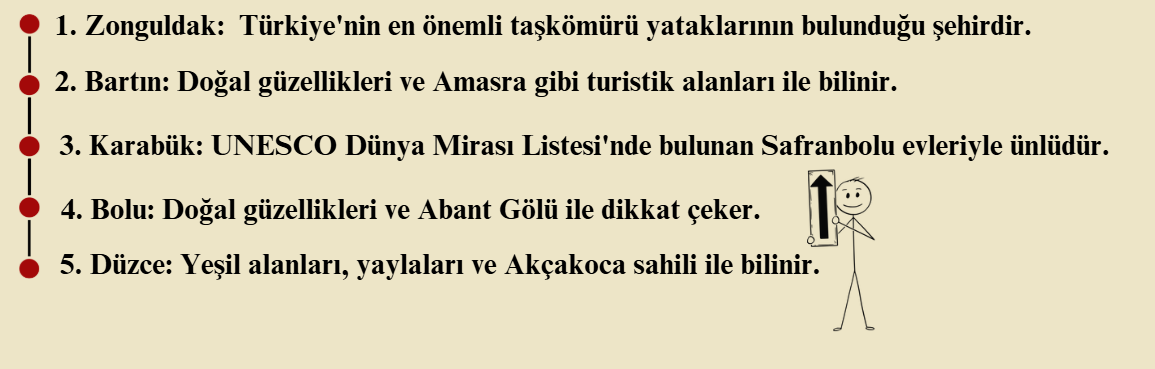
\includegraphics[width=16.04in]{batikaradeniz1}

\paragraph{\texorpdfstring{\emph{\ul{📌Marmara Bölgesinde Bulunan
İller}}}{📌Marmara Bölgesinde Bulunan İller}}\label{marmara-buxf6lgesinde-bulunan-iller}

Marmara Bölgesi, Türkiye'nin en batısında yer alan ve en yoğun nüfusa
sahip olan bölgesidir. Sanayi, ticaret ve turizm alanlarında önemli bir
yere sahiptir. Marmara Bölgesi'nde bulunan iller şunlardır:

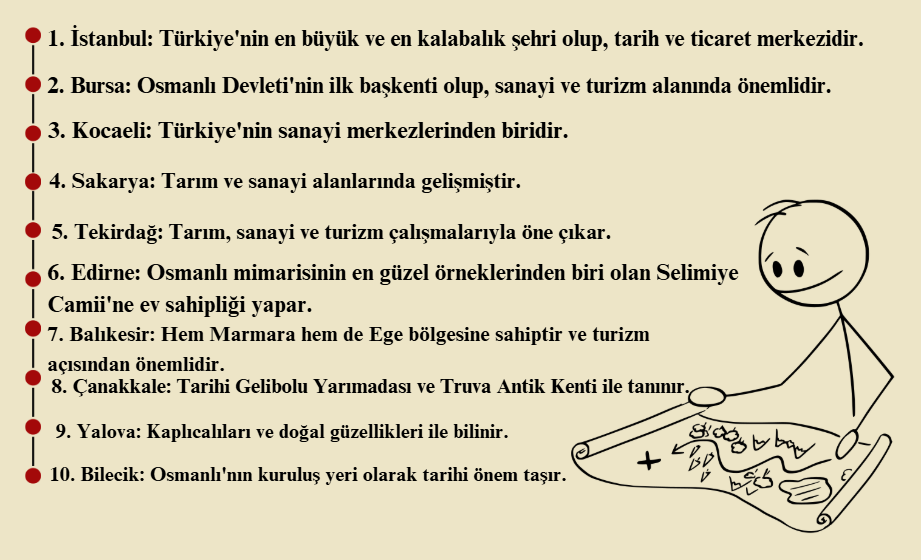
\includegraphics[width=12.79in]{marmara1}

Batı Karadeniz ve Marmara Bölgesi, Türkiye'nin hem doğal hem de ekonomik
bakımdan en önemli iki bölgesidir. Batı Karadeniz, doğal güzellikleri,
ormanları ve denizi ile öne çıkarken; Marmara Bölgesi, sanayi ve
ticaretin kalbi olarak büyük bir ekonomik merkez konumundadır. Bu iki
bölge, Türkiye'nin kalkınmasında çok önemli bir role sahiptir.

\subsubsection{\texorpdfstring{\textbf{\emph{TÜRKİYE HARİTASI ÜZERİNDE
İLLERİN
GÖSTERİMİ}}}{TÜRKİYE HARİTASI ÜZERİNDE İLLERİN GÖSTERİMİ}}\label{tuxfcrkiye-haritasi-uxfczerinde-illerin-guxf6sterimi}

\includegraphics[width=13.93in]{türkiye_haritasi_gosterim}

\subsubsection{\texorpdfstring{\textbf{\emph{BATI KARADENİZ VE MARMARA
BÖLGELERİNDE Kİ İLLERİN SOSYAL AĞ ANALİZİ
}}}{BATI KARADENİZ VE MARMARA BÖLGELERİNDE Kİ İLLERİN SOSYAL AĞ ANALİZİ }}\label{bati-karadeniz-ve-marmara-buxf6lgelerinde-ki-illerin-sosyal-aux11f-analizi}

Blogumun başında bahsettiğim ilk calismam sosyal ag analizi uzerineydi.
Calismamın amaci Türkiye'de bulunan 7 bölgeden 2 tanesinin (Marmara ve
Batı karadeniz) illerinin arasındaki sosyal ağ analiziydi. Sizlere
çalismamda kullandigim kodların guncellenmis ve değiştirilmiş halleriyle
neler yapılabileceğini göstereceğim.

\emph{↪ İlk olarak çalışma yapacağımız konuda kullanacağımız gerekli
kütüphaneleri indirmeliyiz.}

\begin{Shaded}
\begin{Highlighting}[]
\FunctionTok{library}\NormalTok{(igraph)}
\end{Highlighting}
\end{Shaded}

\begin{verbatim}
## 
## Attaching package: 'igraph'
\end{verbatim}

\begin{verbatim}
## The following objects are masked from 'package:stats':
## 
##     decompose, spectrum
\end{verbatim}

\begin{verbatim}
## The following object is masked from 'package:base':
## 
##     union
\end{verbatim}

\begin{Shaded}
\begin{Highlighting}[]
\FunctionTok{library}\NormalTok{(visNetwork)}
\FunctionTok{library}\NormalTok{(ggplot2)}
\end{Highlighting}
\end{Shaded}

\emph{↪ Daha sonra ağ verimizi tanımlamamız gerekiyor. Bunun için veri
seti çekebilir ya da manuel olarak} \emph{girebiliriz. Ben manuel olarak
bağlantılı şehirlerimi tanımlayıp kenar listesi oluşturdum. İşte ↷}

\begin{Shaded}
\begin{Highlighting}[]
\CommentTok{\# Kenar listesi (Şehirler arası bağlantılar)}
\NormalTok{edges }\OtherTok{\textless{}{-}} \FunctionTok{c}\NormalTok{(}\StringTok{"Bolu"}\NormalTok{,}\StringTok{"Duzce"}\NormalTok{, }\StringTok{"Bolu"}\NormalTok{,}\StringTok{"Karabuk"}\NormalTok{, }\StringTok{"Bolu"}\NormalTok{,}\StringTok{"Bartin"}\NormalTok{, }\StringTok{"Bolu"}\NormalTok{,}\StringTok{"Zonguldak"}\NormalTok{, }\StringTok{"Bolu"}\NormalTok{,}\StringTok{"Kastamonu"}\NormalTok{,}
           \StringTok{"Duzce"}\NormalTok{,}\StringTok{"Bolu"}\NormalTok{, }\StringTok{"Duzce"}\NormalTok{,}\StringTok{"Karabuk"}\NormalTok{, }\StringTok{"Duzce"}\NormalTok{,}\StringTok{"Bartin"}\NormalTok{, }\StringTok{"Duzce"}\NormalTok{,}\StringTok{"Zonguldak"}\NormalTok{, }\StringTok{"Duzce"}\NormalTok{,}\StringTok{"Kastamonu"}\NormalTok{,}
           \StringTok{"Karabuk"}\NormalTok{,}\StringTok{"Bolu"}\NormalTok{, }\StringTok{"Karabuk"}\NormalTok{,}\StringTok{"Duzce"}\NormalTok{, }\StringTok{"Karabuk"}\NormalTok{,}\StringTok{"Bartin"}\NormalTok{, }\StringTok{"Karabuk"}\NormalTok{,}\StringTok{"Zonguldak"}\NormalTok{, }\StringTok{"Karabuk"}\NormalTok{,}\StringTok{"Kastamonu"}\NormalTok{,}
           \StringTok{"Bartin"}\NormalTok{,}\StringTok{"Bolu"}\NormalTok{, }\StringTok{"Bartin"}\NormalTok{,}\StringTok{"Duzce"}\NormalTok{, }\StringTok{"Bartin"}\NormalTok{,}\StringTok{"Karabuk"}\NormalTok{, }\StringTok{"Bartin"}\NormalTok{,}\StringTok{"Zonguldak"}\NormalTok{, }\StringTok{"Bartin"}\NormalTok{,}\StringTok{"Kastamonu"}\NormalTok{,}
           \StringTok{"Zonguldak"}\NormalTok{,}\StringTok{"Bolu"}\NormalTok{, }\StringTok{"Zonguldak"}\NormalTok{,}\StringTok{"Duzce"}\NormalTok{, }\StringTok{"Zonguldak"}\NormalTok{,}\StringTok{"Karabuk"}\NormalTok{, }\StringTok{"Zonguldak"}\NormalTok{,}\StringTok{"Bartin"}\NormalTok{, }\StringTok{"Zonguldak"}\NormalTok{,}\StringTok{"Kastamonu"}\NormalTok{,}
           \StringTok{"Kastamonu"}\NormalTok{,}\StringTok{"Bolu"}\NormalTok{, }\StringTok{"Kastamonu"}\NormalTok{,}\StringTok{"Duzce"}\NormalTok{, }\StringTok{"Kastamonu"}\NormalTok{,}\StringTok{"Karabuk"}\NormalTok{, }\StringTok{"Kastamonu"}\NormalTok{,}\StringTok{"Bartin"}\NormalTok{, }\StringTok{"Kastamonu"}\NormalTok{,}\StringTok{"Zonguldak"}\NormalTok{)}

\CommentTok{\# Kenar listesini kullanarak ağ grafiğini oluştur}
\NormalTok{g }\OtherTok{\textless{}{-}} \FunctionTok{graph\_from\_edgelist}\NormalTok{(}\FunctionTok{matrix}\NormalTok{(edges, }\AttributeTok{ncol =} \DecValTok{2}\NormalTok{, }\AttributeTok{byrow =} \ConstantTok{TRUE}\NormalTok{), }\AttributeTok{directed =} \ConstantTok{FALSE}\NormalTok{)}

\CommentTok{\# Düğümlere rastgele koordinatlar atama}
\FunctionTok{set.seed}\NormalTok{(}\DecValTok{42}\NormalTok{)}
\FunctionTok{V}\NormalTok{(g)}\SpecialCharTok{$}\NormalTok{latitude }\OtherTok{\textless{}{-}} \FunctionTok{runif}\NormalTok{(}\FunctionTok{vcount}\NormalTok{(g), }\DecValTok{40}\NormalTok{, }\DecValTok{42}\NormalTok{)}
\FunctionTok{V}\NormalTok{(g)}\SpecialCharTok{$}\NormalTok{longitude }\OtherTok{\textless{}{-}} \FunctionTok{runif}\NormalTok{(}\FunctionTok{vcount}\NormalTok{(g), }\DecValTok{27}\NormalTok{, }\DecValTok{30}\NormalTok{)}

\CommentTok{\# Düğümlere isim verme}
\FunctionTok{V}\NormalTok{(g)}\SpecialCharTok{$}\NormalTok{name }\OtherTok{\textless{}{-}} \FunctionTok{as.character}\NormalTok{(}\FunctionTok{V}\NormalTok{(g))}
\end{Highlighting}
\end{Shaded}

Oluşturduğumuz ağ verilerini grafik çizmek için aşağıdaki kodu
kullanıyoruz. Ortaya temel ağ grafiği çıkacaktır. Grafiğin düğümleri
bordo, kenarlar mavi renkte olacaktır.

\begin{Shaded}
\begin{Highlighting}[]
\CommentTok{\# Görselleştirme için düğüm ve kenar renkleri}
\NormalTok{node\_colors }\OtherTok{\textless{}{-}} \FunctionTok{rep}\NormalTok{(}\StringTok{"\#a30909"}\NormalTok{, }\FunctionTok{vcount}\NormalTok{(g))  }
\NormalTok{edge\_colors }\OtherTok{\textless{}{-}} \FunctionTok{rep}\NormalTok{(}\StringTok{"blue"}\NormalTok{, }\FunctionTok{ecount}\NormalTok{(g))  }
\NormalTok{node\_frame\_colors }\OtherTok{\textless{}{-}} \FunctionTok{rep}\NormalTok{(}\StringTok{"orange"}\NormalTok{, }\FunctionTok{vcount}\NormalTok{(g))  }

\CommentTok{\# Ağın görselleştirilmesi}
\FunctionTok{plot}\NormalTok{(g, }\AttributeTok{edge.arrow.size =} \DecValTok{13}\NormalTok{, }\AttributeTok{vertex.color =}\NormalTok{ node\_colors, }\AttributeTok{vertex.size =} \DecValTok{50}\NormalTok{, }
     \AttributeTok{vertex.frame.color =}\NormalTok{ node\_frame\_colors, }\AttributeTok{vertex.label.color =} \StringTok{"black"}\NormalTok{, }
     \AttributeTok{vertex.label.cex =} \FloatTok{1.2}\NormalTok{, }\AttributeTok{vertex.label.dist =} \DecValTok{2}\NormalTok{, }\AttributeTok{edge.curved =} \FloatTok{0.5}\NormalTok{)}
\end{Highlighting}
\end{Shaded}

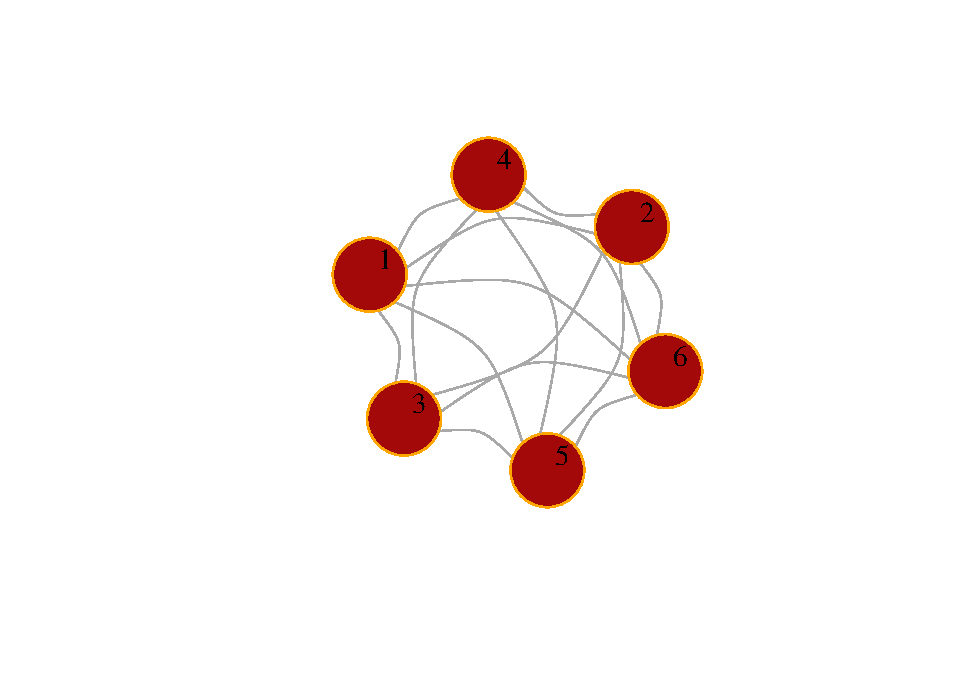
\includegraphics{cigdem_ucar_Rmarkdown_odevi_files/figure-latex/unnamed-chunk-7-1.pdf}

\begin{itemize}
\tightlist
\item
  \emph{Bu kod parçası interaktif bir ağ haritası oluşturur ve bazı
  önemli özellikler içerir:}
\end{itemize}

\texttt{V(g)\$name}: Grafikteki her düğümün (şehrin) adıdır.
\texttt{label}: Düğümlerin üzerine yazılacak isimler belirlenir.
\texttt{lat} ve \texttt{lon}: Düğümlerin koordinat bilgileri (haritada
yerleştirmek için)dir. \texttt{color\ =\ "\#a30909"}: Düğümlerin
varsayılan rengi bordo olarak ayarlanmıştır. \texttt{size\ =\ 10}:
Düğümlerin boyutu 10 punto olarak ayarlanmıştır.

\texttt{visNetwork(nodes,\ edges)} → nodes ve edges kullanarak ağı
oluşturur. \texttt{visNodes(size\ =\ 15,\ shape} = ``dot'', color =
``purple'') → Düğümleri mor renkte ve dot (nokta) şeklinde çizer.
\texttt{visEdges(color\ =\ "grey")} → Kenarları gri renkte gösterir.
\texttt{visOptions(highlightNearest} = TRUE, nodesIdSelection = TRUE)
\texttt{highlightNearest} = TRUE: Bir düğüme tıkladığında, ona bağlı
olan tüm düğümleri vurgular. \texttt{nodesIdSelection} = TRUE: Düğümleri
isimlerine göre seçmeyi sağlar (filtreleme özelliği ekler).
\texttt{visLayout(randomSeed\ =\ 42}, improvedLayout = TRUE)
\texttt{randomSeed\ =\ 42}: Haritanın her çalıştırmada aynı şekilde
düzenlenmesini sağlar bir önceki ağ görselleştirmesinde kullanmadığım
için her çalıştırmamda farktı şekilde düzenlenmektedir.
\texttt{improvedLayout}= TRUE: Daha düzenli bir görselleştirme sağlar.

\begin{Shaded}
\begin{Highlighting}[]
\CommentTok{\# Düğümleri içeren veri çerçevesi}
\NormalTok{nodes }\OtherTok{\textless{}{-}} \FunctionTok{data.frame}\NormalTok{(}
  \AttributeTok{id =} \FunctionTok{V}\NormalTok{(g)}\SpecialCharTok{$}\NormalTok{name, }
  \AttributeTok{label =} \FunctionTok{V}\NormalTok{(g)}\SpecialCharTok{$}\NormalTok{name, }
  \AttributeTok{lat =} \FunctionTok{V}\NormalTok{(g)}\SpecialCharTok{$}\NormalTok{latitude,  }
  \AttributeTok{lon =} \FunctionTok{V}\NormalTok{(g)}\SpecialCharTok{$}\NormalTok{longitude,}
  \AttributeTok{color =} \StringTok{"\#a30909"}\NormalTok{,}
  \AttributeTok{size =} \DecValTok{10}
\NormalTok{)}

\CommentTok{\# Kenarları içeren veri çerçevesi}
\NormalTok{edges }\OtherTok{\textless{}{-}} \FunctionTok{get.data.frame}\NormalTok{(g)}
\end{Highlighting}
\end{Shaded}

\begin{verbatim}
## Warning: `get.data.frame()` was deprecated in igraph 2.0.0.
## i Please use `as_data_frame()` instead.
## This warning is displayed once every 8 hours.
## Call `lifecycle::last_lifecycle_warnings()` to see where this warning was
## generated.
\end{verbatim}

\begin{Shaded}
\begin{Highlighting}[]
\CommentTok{\# Ağ haritası}
\FunctionTok{visNetwork}\NormalTok{(nodes, edges) }\SpecialCharTok{\%\textgreater{}\%}
  \FunctionTok{visNodes}\NormalTok{(}\AttributeTok{size =} \DecValTok{15}\NormalTok{, }\AttributeTok{shape =} \StringTok{"dot"}\NormalTok{, }\AttributeTok{color =} \StringTok{"purple"}\NormalTok{) }\SpecialCharTok{\%\textgreater{}\%}
  \FunctionTok{visEdges}\NormalTok{(}\AttributeTok{color =} \StringTok{"grey"}\NormalTok{) }\SpecialCharTok{\%\textgreater{}\%}
  \FunctionTok{visOptions}\NormalTok{(}\AttributeTok{highlightNearest =} \ConstantTok{TRUE}\NormalTok{, }\AttributeTok{nodesIdSelection =} \ConstantTok{TRUE}\NormalTok{) }\SpecialCharTok{\%\textgreater{}\%}
  \FunctionTok{visLayout}\NormalTok{(}\AttributeTok{randomSeed =} \DecValTok{42}\NormalTok{, }\AttributeTok{improvedLayout =} \ConstantTok{TRUE}\NormalTok{)}
\end{Highlighting}
\end{Shaded}

Yaptığım ilk çalışmamın kısaca özetleyerek bilgilendirdim. şimdi ise
yeni çalışmam hakkında bilgilendireceğim.

\subsubsection{\texorpdfstring{\textbf{\emph{İLLERİN NÜFUS BİLGİLERİ VE
GRAFİKLERİ}}}{İLLERİN NÜFUS BİLGİLERİ VE GRAFİKLERİ}}\label{illerin-nuxfcfus-bilgileri-ve-grafikleri}

İlk çalışmamda Batı karadeniz ve Marmara bölgelerinde bulunan şehirlerin
sosyal ağ analizlerini ele almıştım. Şimdi ise bu şehirler üzerinde son
5 yıl da Nüfus, yaş oranı, cinsiyet oranı gibi konularında
değişiklikleri grafikler üzerinden inceleyeceğiz.

\begin{Shaded}
\begin{Highlighting}[]
\FunctionTok{library}\NormalTok{(tidyverse)}
\end{Highlighting}
\end{Shaded}

\begin{verbatim}
## -- Attaching core tidyverse packages ------------------------ tidyverse 2.0.0 --
## v dplyr     1.1.4     v readr     2.1.5
## v forcats   1.0.0     v stringr   1.5.1
## v lubridate 1.9.4     v tibble    3.2.1
## v purrr     1.0.4     v tidyr     1.3.1
## -- Conflicts ------------------------------------------ tidyverse_conflicts() --
## x lubridate::%--%()      masks igraph::%--%()
## x dplyr::as_data_frame() masks tibble::as_data_frame(), igraph::as_data_frame()
## x purrr::compose()       masks igraph::compose()
## x tidyr::crossing()      masks igraph::crossing()
## x dplyr::filter()        masks stats::filter()
## x dplyr::lag()           masks stats::lag()
## x purrr::simplify()      masks igraph::simplify()
## i Use the conflicted package (<http://conflicted.r-lib.org/>) to force all conflicts to become errors
\end{verbatim}

\begin{Shaded}
\begin{Highlighting}[]
\FunctionTok{library}\NormalTok{(ggplot2)}
\FunctionTok{library}\NormalTok{(scales)}
\end{Highlighting}
\end{Shaded}

\begin{verbatim}
## 
## Attaching package: 'scales'
## 
## The following object is masked from 'package:purrr':
## 
##     discard
## 
## The following object is masked from 'package:readr':
## 
##     col_factor
\end{verbatim}

\begin{Shaded}
\begin{Highlighting}[]
\FunctionTok{library}\NormalTok{(knitr)}
\end{Highlighting}
\end{Shaded}

\subsection{Marmara ve Batı Karadeniz İlleri Nüfus Verileri
(2019-2024)}\label{marmara-ve-batux131-karadeniz-illeri-nuxfcfus-verileri-2019-2024}

Bu kod blogunda, Marmara ve Batı Karadeniz bölgesindeki illerin
2019-2024 yılları arasındaki nüfus bilgilerini girerek görselleştirdik
yani tablo şeklinde bir çıktı alarak belirtilen şehirlerin yıl ve
nüfuslarını görmekteyiz.

\begin{Shaded}
\begin{Highlighting}[]
\CommentTok{\# Nüfus verileri (TÜİK verilerinden örnek olarak alınmıştır)}
\CommentTok{\# Gerçek projenizde güncel ve doğru verileri kullanmalısınız}

\NormalTok{nufus\_verileri }\OtherTok{\textless{}{-}} \FunctionTok{data.frame}\NormalTok{(}
  \AttributeTok{il =} \FunctionTok{c}\NormalTok{(}\StringTok{"Istanbul"}\NormalTok{, }\StringTok{"Bursa"}\NormalTok{, }\StringTok{"Kocaeli"}\NormalTok{, }\StringTok{"Sakarya"}\NormalTok{, }\StringTok{"Tekirdag"}\NormalTok{, }
         \StringTok{"Zonguldak"}\NormalTok{, }\StringTok{"Bartin"}\NormalTok{, }\StringTok{"Karabuk"}\NormalTok{, }\StringTok{"Bolu"}\NormalTok{, }\StringTok{"Duzce"}\NormalTok{),}
  
  \AttributeTok{y2019 =} \FunctionTok{c}\NormalTok{(}\DecValTok{15519267}\NormalTok{, }\DecValTok{3056120}\NormalTok{, }\DecValTok{1953035}\NormalTok{, }\DecValTok{1029650}\NormalTok{, }\DecValTok{1081065}\NormalTok{,}
            \DecValTok{596892}\NormalTok{, }\DecValTok{198999}\NormalTok{, }\DecValTok{248014}\NormalTok{, }\DecValTok{316126}\NormalTok{, }\DecValTok{387844}\NormalTok{),}
  
  \AttributeTok{y2020 =} \FunctionTok{c}\NormalTok{(}\DecValTok{15462452}\NormalTok{, }\DecValTok{3101833}\NormalTok{, }\DecValTok{1997258}\NormalTok{, }\DecValTok{1042649}\NormalTok{, }\DecValTok{1113400}\NormalTok{,}
            \DecValTok{591204}\NormalTok{, }\DecValTok{198979}\NormalTok{, }\DecValTok{244453}\NormalTok{, }\DecValTok{316126}\NormalTok{, }\DecValTok{395679}\NormalTok{),}
  
  \AttributeTok{y2021 =} \FunctionTok{c}\NormalTok{(}\DecValTok{15840900}\NormalTok{, }\DecValTok{3147818}\NormalTok{, }\DecValTok{2033441}\NormalTok{, }\DecValTok{1060876}\NormalTok{, }\DecValTok{1142451}\NormalTok{,}
            \DecValTok{587684}\NormalTok{, }\DecValTok{201711}\NormalTok{, }\DecValTok{242347}\NormalTok{, }\DecValTok{320014}\NormalTok{, }\DecValTok{400976}\NormalTok{),}
  
  \AttributeTok{y2022 =} \FunctionTok{c}\NormalTok{(}\DecValTok{15907951}\NormalTok{, }\DecValTok{3194720}\NormalTok{, }\DecValTok{2079072}\NormalTok{, }\DecValTok{1075420}\NormalTok{, }\DecValTok{1142552}\NormalTok{,}
            \DecValTok{581104}\NormalTok{, }\DecValTok{201061}\NormalTok{, }\DecValTok{240374}\NormalTok{, }\DecValTok{320824}\NormalTok{, }\DecValTok{405106}\NormalTok{),}
  
  \AttributeTok{y2023 =} \FunctionTok{c}\NormalTok{(}\DecValTok{16041602}\NormalTok{, }\DecValTok{3248680}\NormalTok{, }\DecValTok{2122730}\NormalTok{, }\DecValTok{1099631}\NormalTok{, }\DecValTok{1176587}\NormalTok{,}
            \DecValTok{576758}\NormalTok{, }\DecValTok{201293}\NormalTok{, }\DecValTok{239597}\NormalTok{, }\DecValTok{322941}\NormalTok{, }\DecValTok{408623}\NormalTok{),}
  
  \AttributeTok{y2024 =} \FunctionTok{c}\NormalTok{(}\DecValTok{16115795}\NormalTok{, }\DecValTok{3293513}\NormalTok{, }\DecValTok{2159306}\NormalTok{, }\DecValTok{1116925}\NormalTok{, }\DecValTok{1201543}\NormalTok{,}
            \DecValTok{572146}\NormalTok{, }\DecValTok{201508}\NormalTok{, }\DecValTok{238419}\NormalTok{, }\DecValTok{325067}\NormalTok{, }\DecValTok{411249}\NormalTok{)}
\NormalTok{)}

\CommentTok{\# Verileri uzun formata dönüştürme}
\NormalTok{nufus\_uzun }\OtherTok{\textless{}{-}}\NormalTok{ nufus\_verileri }\SpecialCharTok{\%\textgreater{}\%}
  \FunctionTok{pivot\_longer}\NormalTok{(}
    \AttributeTok{cols =} \FunctionTok{starts\_with}\NormalTok{(}\StringTok{"y"}\NormalTok{),}
    \AttributeTok{names\_to =} \StringTok{"yil"}\NormalTok{,}
    \AttributeTok{values\_to =} \StringTok{"nufus"}
\NormalTok{  ) }\SpecialCharTok{\%\textgreater{}\%}
  \FunctionTok{mutate}\NormalTok{(}\AttributeTok{yil =} \FunctionTok{as.integer}\NormalTok{(}\FunctionTok{str\_replace}\NormalTok{(yil, }\StringTok{"y"}\NormalTok{, }\StringTok{""}\NormalTok{)))}

\CommentTok{\# Verileri kontrol etme}
\NormalTok{nufus\_uzun}
\end{Highlighting}
\end{Shaded}

\begin{verbatim}
## # A tibble: 60 x 3
##    il         yil    nufus
##    <chr>    <int>    <dbl>
##  1 Istanbul  2019 15519267
##  2 Istanbul  2020 15462452
##  3 Istanbul  2021 15840900
##  4 Istanbul  2022 15907951
##  5 Istanbul  2023 16041602
##  6 Istanbul  2024 16115795
##  7 Bursa     2019  3056120
##  8 Bursa     2020  3101833
##  9 Bursa     2021  3147818
## 10 Bursa     2022  3194720
## # i 50 more rows
\end{verbatim}

\subsection{📈 Tüm İllerin Nüfus
Grafiği}\label{tuxfcm-illerin-nuxfcfus-grafiux11fi}

Burada iki bölgeye ait tüm illerin nüfus değişimini gösteren çizgi
grafiğini elde etmek amaçlanmıştır.

\begin{Shaded}
\begin{Highlighting}[]
\CommentTok{\# Tüm illerin nüfus değişimini gösteren çizgi grafiği}
\FunctionTok{ggplot}\NormalTok{(nufus\_uzun, }\FunctionTok{aes}\NormalTok{(}\AttributeTok{x =}\NormalTok{ yil, }\AttributeTok{y =}\NormalTok{ nufus, }\AttributeTok{color =}\NormalTok{ il, }\AttributeTok{group =}\NormalTok{ il)) }\SpecialCharTok{+}
  \FunctionTok{geom\_line}\NormalTok{(}\AttributeTok{linewidth =} \DecValTok{1}\NormalTok{) }\SpecialCharTok{+}
  \FunctionTok{geom\_point}\NormalTok{(}\AttributeTok{size =} \DecValTok{2}\NormalTok{) }\SpecialCharTok{+}
  \FunctionTok{scale\_y\_continuous}\NormalTok{(}\AttributeTok{labels =} \FunctionTok{label\_comma}\NormalTok{()) }\SpecialCharTok{+}
  \FunctionTok{scale\_x\_continuous}\NormalTok{(}\AttributeTok{breaks =} \DecValTok{2019}\SpecialCharTok{:}\DecValTok{2024}\NormalTok{) }\SpecialCharTok{+}
  \FunctionTok{labs}\NormalTok{(}
    \AttributeTok{title =} \StringTok{"Marmara ve Bati Karadeniz Illeri Nufus Degisimi (2019{-}2024)"}\NormalTok{,}
    \AttributeTok{subtitle =} \StringTok{"TUIK verileri baz alinmistir"}\NormalTok{,}
    \AttributeTok{x =} \StringTok{"Yil"}\NormalTok{,}
    \AttributeTok{y =} \StringTok{"Nufus"}\NormalTok{,}
    \AttributeTok{color =} \StringTok{"Il"}
\NormalTok{  ) }\SpecialCharTok{+}
  \FunctionTok{theme\_minimal}\NormalTok{() }\SpecialCharTok{+}
  \FunctionTok{theme}\NormalTok{(}
    \AttributeTok{legend.position =} \StringTok{"right"}\NormalTok{,}
    \AttributeTok{plot.title =} \FunctionTok{element\_text}\NormalTok{(}\AttributeTok{face =} \StringTok{"bold"}\NormalTok{),}
    \AttributeTok{axis.text.x =} \FunctionTok{element\_text}\NormalTok{(}\AttributeTok{angle =} \DecValTok{0}\NormalTok{)}
\NormalTok{  )}
\end{Highlighting}
\end{Shaded}

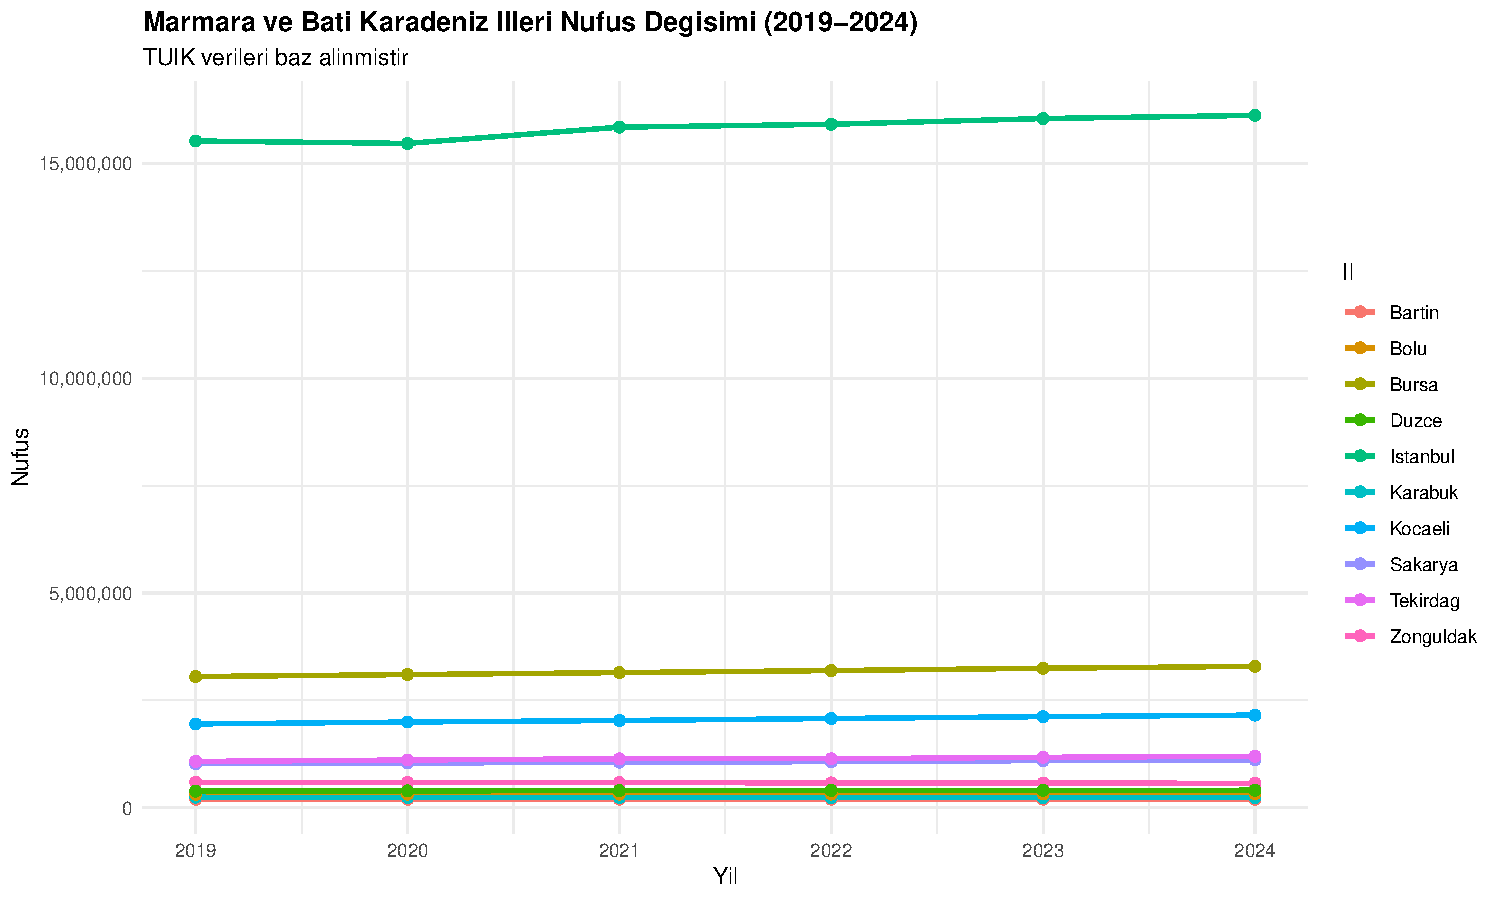
\includegraphics{cigdem_ucar_Rmarkdown_odevi_files/figure-latex/tum-iller-grafik-1.pdf}

Çizgi grafiğini incelediğimizde ⇑ İstanbul'un nüfusu diğer illere göre
çok yüksek olduğundan, grafikte diğer illerin değişimini görmekte
zorlanıyoruz. Bu nedenle, aşağıda İstanbul hariç diğer illerin nüfus
değişimini gösteren çizgi grafiğini oluşturdum.

\begin{Shaded}
\begin{Highlighting}[]
\NormalTok{nufus\_uzun }\SpecialCharTok{\%\textgreater{}\%}
  \FunctionTok{filter}\NormalTok{(il }\SpecialCharTok{!=} \StringTok{"Istanbul"}\NormalTok{) }\SpecialCharTok{\%\textgreater{}\%}
  \FunctionTok{ggplot}\NormalTok{(}\FunctionTok{aes}\NormalTok{(}\AttributeTok{x =}\NormalTok{ yil, }\AttributeTok{y =}\NormalTok{ nufus, }\AttributeTok{color =}\NormalTok{ il, }\AttributeTok{group =}\NormalTok{ il)) }\SpecialCharTok{+}
  \FunctionTok{geom\_line}\NormalTok{(}\AttributeTok{linewidth =} \DecValTok{1}\NormalTok{) }\SpecialCharTok{+}
  \FunctionTok{geom\_point}\NormalTok{(}\AttributeTok{size =} \DecValTok{2}\NormalTok{) }\SpecialCharTok{+}
  \FunctionTok{scale\_y\_continuous}\NormalTok{(}\AttributeTok{labels =} \FunctionTok{label\_comma}\NormalTok{()) }\SpecialCharTok{+}
  \FunctionTok{scale\_x\_continuous}\NormalTok{(}\AttributeTok{breaks =} \DecValTok{2019}\SpecialCharTok{:}\DecValTok{2024}\NormalTok{) }\SpecialCharTok{+}
  \FunctionTok{labs}\NormalTok{(}
    \AttributeTok{title =} \StringTok{"Marmara ve Bati Karadeniz Illeri Nufus Degisimi (2019{-}2024)"}\NormalTok{,}
    \AttributeTok{subtitle =} \StringTok{"Istanbul haric"}\NormalTok{,}
    \AttributeTok{x =} \StringTok{"Yil"}\NormalTok{,}
    \AttributeTok{y =} \StringTok{"Nufus"}\NormalTok{,}
    \AttributeTok{color =} \StringTok{"Il"}
\NormalTok{  ) }\SpecialCharTok{+}
  \FunctionTok{theme\_minimal}\NormalTok{() }\SpecialCharTok{+}
  \FunctionTok{theme}\NormalTok{(}
    \AttributeTok{legend.position =} \StringTok{"right"}\NormalTok{,}
    \AttributeTok{plot.title =} \FunctionTok{element\_text}\NormalTok{(}\AttributeTok{face =} \StringTok{"bold"}\NormalTok{),}
    \AttributeTok{axis.text.x =} \FunctionTok{element\_text}\NormalTok{(}\AttributeTok{angle =} \DecValTok{0}\NormalTok{)}
\NormalTok{  )}
\end{Highlighting}
\end{Shaded}

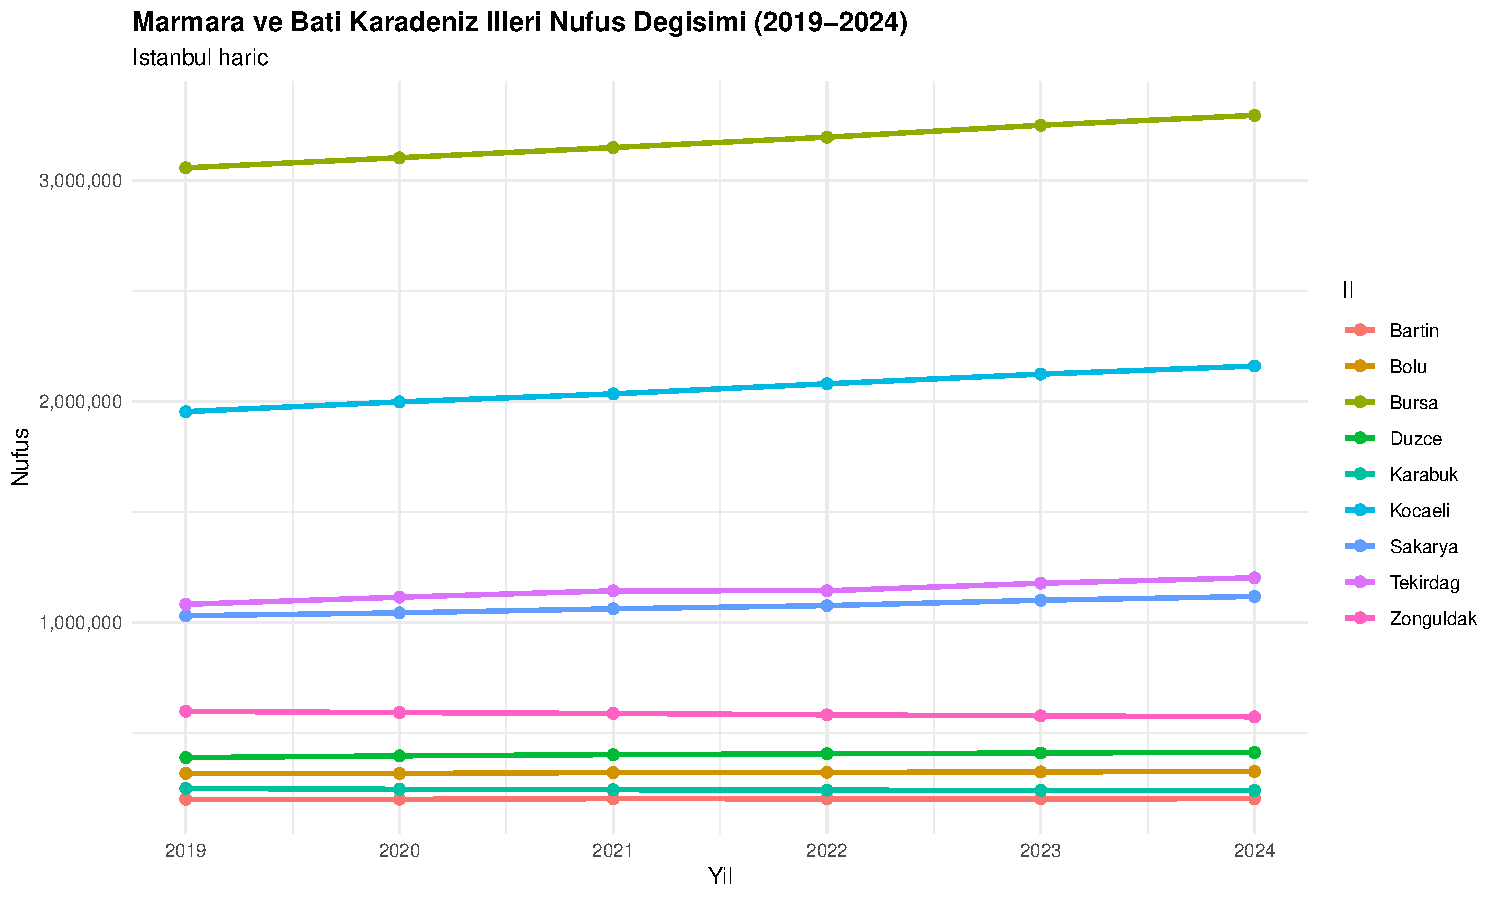
\includegraphics{cigdem_ucar_Rmarkdown_odevi_files/figure-latex/istanbul-haric-grafik-1.pdf}

\subsection{📈 Yüzdesel Değişim
Grafiği}\label{yuxfczdesel-deux11fiux15fim-grafiux11fi}

Her ilin 2019'dan 2024'e kadar olan yüzdesel değişimini çizgisel
grafikte değil de nokta grafiğinde görelim:

\begin{Shaded}
\begin{Highlighting}[]
\NormalTok{yuzdesel\_degisim }\OtherTok{\textless{}{-}}\NormalTok{ nufus\_uzun }\SpecialCharTok{\%\textgreater{}\%}
  \FunctionTok{group\_by}\NormalTok{(il) }\SpecialCharTok{\%\textgreater{}\%}
  \FunctionTok{mutate}\NormalTok{(}
    \AttributeTok{baz\_yil =} \FunctionTok{first}\NormalTok{(nufus),}
    \AttributeTok{yuzde\_degisim =}\NormalTok{ (nufus }\SpecialCharTok{/}\NormalTok{ baz\_yil }\SpecialCharTok{{-}} \DecValTok{1}\NormalTok{) }\SpecialCharTok{*} \DecValTok{100}
\NormalTok{  )}

\FunctionTok{ggplot}\NormalTok{(yuzdesel\_degisim, }\FunctionTok{aes}\NormalTok{(}\AttributeTok{x =}\NormalTok{ yil, }\AttributeTok{y =}\NormalTok{ yuzde\_degisim, }\AttributeTok{color =}\NormalTok{ il, }\AttributeTok{group =}\NormalTok{ il)) }\SpecialCharTok{+}
  \FunctionTok{geom\_point}\NormalTok{(}\AttributeTok{size =} \DecValTok{3}\NormalTok{, }\AttributeTok{alpha =} \FloatTok{0.8}\NormalTok{) }\SpecialCharTok{+}  
  \FunctionTok{geom\_line}\NormalTok{(}\AttributeTok{linetype =} \StringTok{"dotted"}\NormalTok{, }\AttributeTok{linewidth =} \FloatTok{0.5}\NormalTok{, }\AttributeTok{alpha =} \FloatTok{0.6}\NormalTok{) }\SpecialCharTok{+}
  \FunctionTok{scale\_y\_continuous}\NormalTok{(}\AttributeTok{labels =} \ControlFlowTok{function}\NormalTok{(x) }\FunctionTok{paste0}\NormalTok{(x, }\StringTok{"\%"}\NormalTok{)) }\SpecialCharTok{+}
  \FunctionTok{scale\_x\_continuous}\NormalTok{(}\AttributeTok{breaks =} \DecValTok{2019}\SpecialCharTok{:}\DecValTok{2024}\NormalTok{) }\SpecialCharTok{+}
  \FunctionTok{labs}\NormalTok{(}
    \AttributeTok{title =} \StringTok{"Marmara ve Batı Karadeniz İlleri Nüfus Değişim Oranı (2019{-}2024)"}\NormalTok{,}
    \AttributeTok{subtitle =} \StringTok{"2019 baz yıl olarak alınmıştır"}\NormalTok{,}
    \AttributeTok{x =} \StringTok{"Yıl"}\NormalTok{,}
    \AttributeTok{y =} \StringTok{"Değişim Oranı (\%)"}\NormalTok{,}
    \AttributeTok{color =} \StringTok{"İl"}
\NormalTok{  ) }\SpecialCharTok{+}
  
  \FunctionTok{theme}\NormalTok{(}
    \AttributeTok{legend.position =} \StringTok{"right"}\NormalTok{,}
    \AttributeTok{plot.title =} \FunctionTok{element\_text}\NormalTok{(}\AttributeTok{face =} \StringTok{"bold"}\NormalTok{),}
    \AttributeTok{axis.text.x =} \FunctionTok{element\_text}\NormalTok{(}\AttributeTok{angle =} \DecValTok{0}\NormalTok{)}
\NormalTok{  )}
\end{Highlighting}
\end{Shaded}

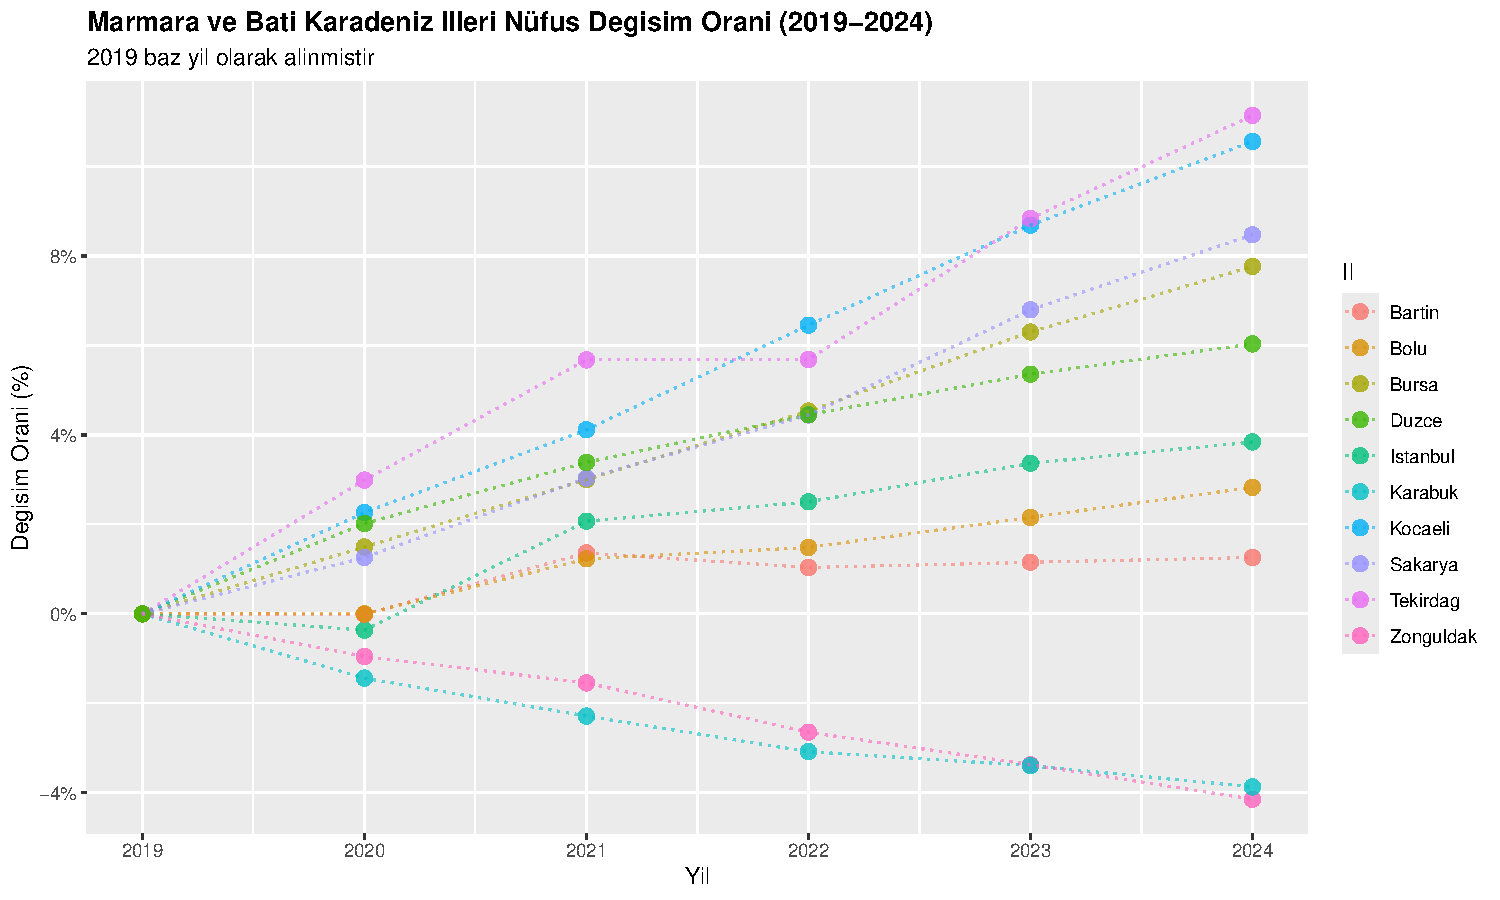
\includegraphics{cigdem_ucar_Rmarkdown_odevi_files/figure-latex/yuzdesel-degisim-1.pdf}

Çıktısını aldığım nokta grafiğinde illerin yıllar bazındaki
değişimlerini detaylı bir şekilde incelemekteyiz.

\subsection{Nüfus Verileri Tablosu}\label{nuxfcfus-verileri-tablosu}

Burada belirtmiş olduğum tabloda yukarıdaki verileri çekerek aşağıdaki
kod bloğuyla satır sütün şeklinde bir tablo oluşturdum.

\begin{Shaded}
\begin{Highlighting}[]
\CommentTok{\# Nüfus verileri tablosu}
\NormalTok{nufus\_verileri }\SpecialCharTok{\%\textgreater{}\%}
  \FunctionTok{kable}\NormalTok{(}
    \AttributeTok{caption =} \StringTok{"Marmara ve Batı Karadeniz İlleri Nüfus Verileri (2019{-}2024)"}\NormalTok{,}
    \AttributeTok{format.args =} \FunctionTok{list}\NormalTok{(}\AttributeTok{big.mark =} \StringTok{"."}\NormalTok{, }\AttributeTok{decimal.mark =} \StringTok{","}\NormalTok{),}
    \AttributeTok{col.names =} \FunctionTok{c}\NormalTok{(}\StringTok{"İl"}\NormalTok{, }\StringTok{"2019"}\NormalTok{, }\StringTok{"2020"}\NormalTok{, }\StringTok{"2021"}\NormalTok{, }\StringTok{"2022"}\NormalTok{, }\StringTok{"2023"}\NormalTok{, }\StringTok{"2024"}\NormalTok{)}
\NormalTok{  )}
\end{Highlighting}
\end{Shaded}

\begin{longtable}[]{@{}
  >{\raggedright\arraybackslash}p{(\columnwidth - 12\tabcolsep) * \real{0.1316}}
  >{\raggedleft\arraybackslash}p{(\columnwidth - 12\tabcolsep) * \real{0.1447}}
  >{\raggedleft\arraybackslash}p{(\columnwidth - 12\tabcolsep) * \real{0.1447}}
  >{\raggedleft\arraybackslash}p{(\columnwidth - 12\tabcolsep) * \real{0.1447}}
  >{\raggedleft\arraybackslash}p{(\columnwidth - 12\tabcolsep) * \real{0.1447}}
  >{\raggedleft\arraybackslash}p{(\columnwidth - 12\tabcolsep) * \real{0.1447}}
  >{\raggedleft\arraybackslash}p{(\columnwidth - 12\tabcolsep) * \real{0.1447}}@{}}
\caption{Marmara ve Batı Karadeniz İlleri Nüfus Verileri
(2019-2024)}\tabularnewline
\toprule\noalign{}
\begin{minipage}[b]{\linewidth}\raggedright
İl
\end{minipage} & \begin{minipage}[b]{\linewidth}\raggedleft
2019
\end{minipage} & \begin{minipage}[b]{\linewidth}\raggedleft
2020
\end{minipage} & \begin{minipage}[b]{\linewidth}\raggedleft
2021
\end{minipage} & \begin{minipage}[b]{\linewidth}\raggedleft
2022
\end{minipage} & \begin{minipage}[b]{\linewidth}\raggedleft
2023
\end{minipage} & \begin{minipage}[b]{\linewidth}\raggedleft
2024
\end{minipage} \\
\midrule\noalign{}
\endfirsthead
\toprule\noalign{}
\begin{minipage}[b]{\linewidth}\raggedright
İl
\end{minipage} & \begin{minipage}[b]{\linewidth}\raggedleft
2019
\end{minipage} & \begin{minipage}[b]{\linewidth}\raggedleft
2020
\end{minipage} & \begin{minipage}[b]{\linewidth}\raggedleft
2021
\end{minipage} & \begin{minipage}[b]{\linewidth}\raggedleft
2022
\end{minipage} & \begin{minipage}[b]{\linewidth}\raggedleft
2023
\end{minipage} & \begin{minipage}[b]{\linewidth}\raggedleft
2024
\end{minipage} \\
\midrule\noalign{}
\endhead
\bottomrule\noalign{}
\endlastfoot
Istanbul & 15.519.267 & 15.462.452 & 15.840.900 & 15.907.951 &
16.041.602 & 16.115.795 \\
Bursa & 3.056.120 & 3.101.833 & 3.147.818 & 3.194.720 & 3.248.680 &
3.293.513 \\
Kocaeli & 1.953.035 & 1.997.258 & 2.033.441 & 2.079.072 & 2.122.730 &
2.159.306 \\
Sakarya & 1.029.650 & 1.042.649 & 1.060.876 & 1.075.420 & 1.099.631 &
1.116.925 \\
Tekirdag & 1.081.065 & 1.113.400 & 1.142.451 & 1.142.552 & 1.176.587 &
1.201.543 \\
Zonguldak & 596.892 & 591.204 & 587.684 & 581.104 & 576.758 & 572.146 \\
Bartin & 198.999 & 198.979 & 201.711 & 201.061 & 201.293 & 201.508 \\
Karabuk & 248.014 & 244.453 & 242.347 & 240.374 & 239.597 & 238.419 \\
Bolu & 316.126 & 316.126 & 320.014 & 320.824 & 322.941 & 325.067 \\
Duzce & 387.844 & 395.679 & 400.976 & 405.106 & 408.623 & 411.249 \\
\end{longtable}

Çıktısı olan tabloyu kodlarla oluşturduğumu belirtmiştim. Bir de manuel
olarak aynı tabloyu oluşturacağım.

\begin{longtable}[]{@{}
  >{\raggedright\arraybackslash}p{(\columnwidth - 12\tabcolsep) * \real{0.1538}}
  >{\raggedleft\arraybackslash}p{(\columnwidth - 12\tabcolsep) * \real{0.1538}}
  >{\raggedleft\arraybackslash}p{(\columnwidth - 12\tabcolsep) * \real{0.1410}}
  >{\raggedleft\arraybackslash}p{(\columnwidth - 12\tabcolsep) * \real{0.1410}}
  >{\raggedleft\arraybackslash}p{(\columnwidth - 12\tabcolsep) * \real{0.1410}}
  >{\raggedleft\arraybackslash}p{(\columnwidth - 12\tabcolsep) * \real{0.1410}}
  >{\raggedright\arraybackslash}p{(\columnwidth - 12\tabcolsep) * \real{0.1282}}@{}}
\toprule\noalign{}
\begin{minipage}[b]{\linewidth}\raggedright
İl
\end{minipage} & \begin{minipage}[b]{\linewidth}\raggedleft
2019
\end{minipage} & \begin{minipage}[b]{\linewidth}\raggedleft
2020
\end{minipage} & \begin{minipage}[b]{\linewidth}\raggedleft
2021
\end{minipage} & \begin{minipage}[b]{\linewidth}\raggedleft
2022
\end{minipage} & \begin{minipage}[b]{\linewidth}\raggedleft
2023
\end{minipage} & \begin{minipage}[b]{\linewidth}\raggedright
2024
\end{minipage} \\
\midrule\noalign{}
\endhead
\bottomrule\noalign{}
\endlastfoot
İstanbul & 15.519.267 & 15.462.452 & 15.840.900 & 15.907.951 &
16.041.602 & 16.115.795 \\
:----------- & -----------: & ----------: & ----------: & ----------: &
----------: & ---------- \\
Bursa & 3.056.120 & 3.101.833 & 3.147.818 & 3.194.720 & 3.248.680 &
3.293.513 \\
:----------- & -----------: & ----------: & ----------: & ----------: &
----------: & ---------- \\
Kocaeli & 1.953.035 & 1.997.258 & 2.033.441 & 2.079.072 & 2.122.730 &
2.159.306 \\
:----------- & -----------: & ----------: & ----------: & ----------: &
----------: & ---------- \\
Sakarya & 1.029.650 & 1.042.649 & 1.060.876 & 1.075.420 & 1.099.631 &
1.116.925 \\
:----------- & -----------: & ----------: & ----------: & ----------: &
----------: & ---------- \\
Tekirdağ & 1.081.065 & 1.113.400 & 1.142.451 & 1.142.552 & 1.176.587 &
1.201.543 \\
:----------- & -----------: & ----------: & ----------: & ----------: &
----------: & ---------- \\
Zonguldak & 596.892 & 591.204 & 587.684 & 581.104 & 576.758 & 572.146 \\
:----------- & -----------: & ----------: & ----------: & ----------: &
----------: & ---------- \\
Bartın & 198.999 & 198.979 & 201.711 & 201.061 & 201.293 & 201.508 \\
:----------- & -----------: & ----------: & ----------: & ----------: &
----------: & ---------- \\
Karabük & 248.014 & 244.453 & 242.347 & 240.374 & 239.597 & 238.419 \\
:----------- & -----------: & ----------: & ----------: & ----------: &
----------: & ---------- \\
Bolu & 316.126 & 316.126 & 320.014 & 320.824 & 322.941 & 325.067 \\
:----------- & -----------: & ----------: & ----------: & ----------: &
----------: & ---------- \\
Düzce & 387.844 & 395.679 & 400.976 & 405.106 & 408.623 & 411.249 \\
\end{longtable}

Bu grafikler ve tablolar, Marmara ve Batı Karadeniz bölgesindeki illerin
2019-2024 yılları arasındaki nüfus değişimini göstermektedir. Görüldüğü
üzere, Marmara bölgesindeki illerin çoğu artış gösterirken, Batı
Karadeniz bölgesindeki bazı illerde azalma eğilimi görülmektedir.

\subsection{Marmara ve Batı Karadeniz İlleri Yaş Dağılımı
(2024)}\label{marmara-ve-batux131-karadeniz-illeri-yaux15f-daux11fux131lux131mux131-2024}

Bu dokümanda, Marmara ve Batı Karadeniz bölgesindeki illerin yaş
dağılımı pasta grafikleri ile görselleştirilmiştir.

\begin{Shaded}
\begin{Highlighting}[]
\NormalTok{yas\_verileri }\OtherTok{\textless{}{-}} \FunctionTok{data.frame}\NormalTok{(}
  \AttributeTok{il =} \FunctionTok{c}\NormalTok{(}\StringTok{"Istanbul"}\NormalTok{, }\StringTok{"Bursa"}\NormalTok{, }\StringTok{"Kocaeli"}\NormalTok{, }\StringTok{"Sakarya"}\NormalTok{, }\StringTok{"Tekirdag"}\NormalTok{, }
         \StringTok{"Zonguldak"}\NormalTok{, }\StringTok{"Bartin"}\NormalTok{, }\StringTok{"Karabuk"}\NormalTok{, }\StringTok{"Bolu"}\NormalTok{, }\StringTok{"Duzce"}\NormalTok{),}
  
  \AttributeTok{yas\_0\_14 =} \FunctionTok{c}\NormalTok{(}\FloatTok{23.5}\NormalTok{, }\FloatTok{22.3}\NormalTok{, }\FloatTok{23.1}\NormalTok{, }\FloatTok{22.8}\NormalTok{, }\FloatTok{21.5}\NormalTok{,}
               \FloatTok{18.2}\NormalTok{, }\FloatTok{17.5}\NormalTok{, }\FloatTok{17.3}\NormalTok{, }\FloatTok{18.1}\NormalTok{, }\FloatTok{21.2}\NormalTok{),}
  
  \AttributeTok{yas\_15\_24 =} \FunctionTok{c}\NormalTok{(}\FloatTok{15.8}\NormalTok{, }\FloatTok{15.2}\NormalTok{, }\FloatTok{15.7}\NormalTok{, }\FloatTok{15.3}\NormalTok{, }\FloatTok{15.0}\NormalTok{,}
                \FloatTok{13.5}\NormalTok{, }\FloatTok{13.2}\NormalTok{, }\FloatTok{12.7}\NormalTok{, }\FloatTok{14.0}\NormalTok{, }\FloatTok{15.3}\NormalTok{),}
  
  \AttributeTok{yas\_25\_44 =} \FunctionTok{c}\NormalTok{(}\FloatTok{34.2}\NormalTok{, }\FloatTok{32.8}\NormalTok{, }\FloatTok{33.1}\NormalTok{, }\FloatTok{31.7}\NormalTok{, }\FloatTok{32.5}\NormalTok{,}
                \FloatTok{29.2}\NormalTok{, }\FloatTok{27.5}\NormalTok{, }\FloatTok{27.3}\NormalTok{, }\FloatTok{28.4}\NormalTok{, }\FloatTok{30.2}\NormalTok{),}
  
  \AttributeTok{yas\_45\_64 =} \FunctionTok{c}\NormalTok{(}\FloatTok{19.7}\NormalTok{, }\FloatTok{21.3}\NormalTok{, }\FloatTok{20.5}\NormalTok{, }\FloatTok{21.4}\NormalTok{, }\FloatTok{22.5}\NormalTok{,}
                \FloatTok{25.3}\NormalTok{, }\FloatTok{26.5}\NormalTok{, }\FloatTok{26.7}\NormalTok{, }\FloatTok{25.2}\NormalTok{, }\FloatTok{22.8}\NormalTok{),}
  
  \AttributeTok{yas\_65\_ustu =} \FunctionTok{c}\NormalTok{(}\FloatTok{6.8}\NormalTok{, }\FloatTok{8.4}\NormalTok{, }\FloatTok{7.6}\NormalTok{, }\FloatTok{8.8}\NormalTok{, }\FloatTok{8.5}\NormalTok{,}
                  \FloatTok{13.8}\NormalTok{, }\FloatTok{15.3}\NormalTok{, }\FloatTok{16.0}\NormalTok{, }\FloatTok{14.3}\NormalTok{, }\FloatTok{10.5}\NormalTok{)}
\NormalTok{)}

\CommentTok{\# Verileri uzun formata donusturme}
\NormalTok{yas\_uzun }\OtherTok{\textless{}{-}}\NormalTok{ yas\_verileri }\SpecialCharTok{\%\textgreater{}\%}
  \FunctionTok{pivot\_longer}\NormalTok{(}
    \AttributeTok{cols =} \FunctionTok{starts\_with}\NormalTok{(}\StringTok{"yas\_"}\NormalTok{),}
    \AttributeTok{names\_to =} \StringTok{"yas\_grubu"}\NormalTok{,}
    \AttributeTok{values\_to =} \StringTok{"yuzde"}
\NormalTok{  ) }\SpecialCharTok{\%\textgreater{}\%}
  \FunctionTok{mutate}\NormalTok{(}
    \AttributeTok{yas\_grubu =} \FunctionTok{case\_when}\NormalTok{(}
\NormalTok{      yas\_grubu }\SpecialCharTok{==} \StringTok{"yas\_0\_14"} \SpecialCharTok{\textasciitilde{}} \StringTok{"0{-}14 Yas"}\NormalTok{,}
\NormalTok{      yas\_grubu }\SpecialCharTok{==} \StringTok{"yas\_15\_24"} \SpecialCharTok{\textasciitilde{}} \StringTok{"15{-}24 Yas"}\NormalTok{,}
\NormalTok{      yas\_grubu }\SpecialCharTok{==} \StringTok{"yas\_25\_44"} \SpecialCharTok{\textasciitilde{}} \StringTok{"25{-}44 Yas"}\NormalTok{,}
\NormalTok{      yas\_grubu }\SpecialCharTok{==} \StringTok{"yas\_45\_64"} \SpecialCharTok{\textasciitilde{}} \StringTok{"45{-}64 Yas"}\NormalTok{,}
\NormalTok{      yas\_grubu }\SpecialCharTok{==} \StringTok{"yas\_65\_ustu"} \SpecialCharTok{\textasciitilde{}} \StringTok{"65+ Yas"}
\NormalTok{    )}
\NormalTok{  )}

\CommentTok{\# Verileri kontrol etme}
\FunctionTok{head}\NormalTok{(yas\_uzun)}
\end{Highlighting}
\end{Shaded}

\begin{verbatim}
## # A tibble: 6 x 3
##   il       yas_grubu yuzde
##   <chr>    <chr>     <dbl>
## 1 Istanbul 0-14 Yas   23.5
## 2 Istanbul 15-24 Yas  15.8
## 3 Istanbul 25-44 Yas  34.2
## 4 Istanbul 45-64 Yas  19.7
## 5 Istanbul 65+ Yas     6.8
## 6 Bursa    0-14 Yas   22.3
\end{verbatim}

\subsection{İller İçin Pasta
Grafikleri}\label{iller-iuxe7in-pasta-grafikleri}

Her il için ayrı bir pasta grafiği oluşturarak illerin yaş dağılımlarını
incelemeyi amaçladım.

\begin{Shaded}
\begin{Highlighting}[]
\NormalTok{yas\_renkleri }\OtherTok{\textless{}{-}} \FunctionTok{c}\NormalTok{(}\StringTok{"0{-}14 Yas"} \OtherTok{=} \StringTok{"\#a20a0a"}\NormalTok{, }
                 \StringTok{"15{-}24 Yas"} \OtherTok{=} \StringTok{"\#ffde59"}\NormalTok{, }
                 \StringTok{"25{-}44 Yas"} \OtherTok{=} \StringTok{"\#8da0cb"}\NormalTok{, }
                 \StringTok{"45{-}64 Yas"} \OtherTok{=} \StringTok{"\#e78ac3"}\NormalTok{, }
                 \StringTok{"65+ Yas"} \OtherTok{=} \StringTok{"\#ade196"}\NormalTok{)}


\FunctionTok{ggplot}\NormalTok{(yas\_uzun, }\FunctionTok{aes}\NormalTok{(}\AttributeTok{x =} \StringTok{""}\NormalTok{, }\AttributeTok{y =}\NormalTok{ yuzde, }\AttributeTok{fill =}\NormalTok{ yas\_grubu)) }\SpecialCharTok{+}
  \FunctionTok{geom\_bar}\NormalTok{(}\AttributeTok{stat =} \StringTok{"identity"}\NormalTok{, }\AttributeTok{width =} \DecValTok{1}\NormalTok{) }\SpecialCharTok{+}
  \FunctionTok{coord\_polar}\NormalTok{(}\StringTok{"y"}\NormalTok{, }\AttributeTok{start =} \DecValTok{0}\NormalTok{) }\SpecialCharTok{+}
  \FunctionTok{scale\_fill\_manual}\NormalTok{(}\AttributeTok{values =}\NormalTok{ yas\_renkleri) }\SpecialCharTok{+}
  \FunctionTok{labs}\NormalTok{(}
    \AttributeTok{title =} \StringTok{"Marmara ve Bati Karadeniz Illerinin Yas Dagilimi (2024)"}\NormalTok{,}
    \AttributeTok{fill =} \StringTok{"Yas Grubu"}
\NormalTok{  ) }\SpecialCharTok{+}
  \FunctionTok{theme\_void}\NormalTok{() }\SpecialCharTok{+}
  \FunctionTok{theme}\NormalTok{(}
    \AttributeTok{legend.position =} \StringTok{"bottom"}\NormalTok{,}
    \AttributeTok{plot.title =} \FunctionTok{element\_text}\NormalTok{(}\AttributeTok{hjust =} \FloatTok{0.5}\NormalTok{, }\AttributeTok{face =} \StringTok{"bold"}\NormalTok{),}
    \AttributeTok{strip.text =} \FunctionTok{element\_text}\NormalTok{(}\AttributeTok{size =} \DecValTok{12}\NormalTok{, }\AttributeTok{face =} \StringTok{"bold"}\NormalTok{)}
\NormalTok{  ) }\SpecialCharTok{+}
  \FunctionTok{facet\_wrap}\NormalTok{(}\SpecialCharTok{\textasciitilde{}}\NormalTok{ il, }\AttributeTok{ncol =} \DecValTok{3}\NormalTok{)}
\end{Highlighting}
\end{Shaded}

\begin{center}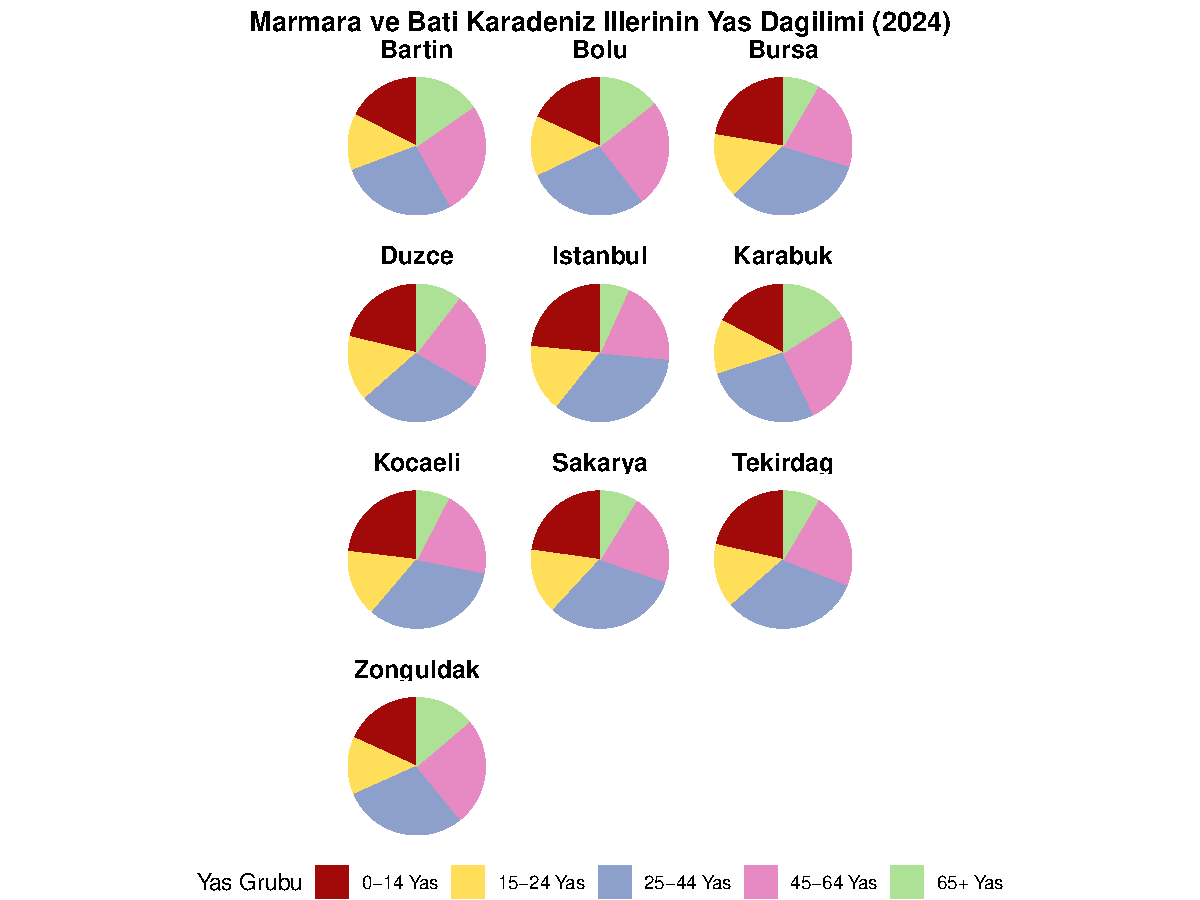
\includegraphics[width=0.8\linewidth]{cigdem_ucar_Rmarkdown_odevi_files/figure-latex/pasta-grafikleri-1} \end{center}

\subsection{Her İl İçin Ayrı Pasta
Grafikleri}\label{her-il-iuxe7in-ayrux131-pasta-grafikleri}

Bu kodu kullanarak istediğimiz şehir için detaylı bir şekilde pasta
grafiğini görebiliriz. İşte seçili iller için daha detaylı grafikleri
görelim:

\begin{Shaded}
\begin{Highlighting}[]
\CommentTok{\# Secili iller (Marmara\textquotesingle{}dan ve Bati Karadeniz\textquotesingle{}den ornekler)}
\NormalTok{secili\_iller }\OtherTok{\textless{}{-}} \FunctionTok{c}\NormalTok{(}\StringTok{"Istanbul"}\NormalTok{, }\StringTok{"Bursa"}\NormalTok{, }\StringTok{"Kocaeli"}\NormalTok{, }\StringTok{"Duzce"}\NormalTok{)}

\CommentTok{\# Secili iller icin pasta grafigi olusturma}
\NormalTok{yas\_uzun }\SpecialCharTok{\%\textgreater{}\%}
  \FunctionTok{filter}\NormalTok{(il }\SpecialCharTok{\%in\%}\NormalTok{ secili\_iller) }\SpecialCharTok{\%\textgreater{}\%}
  \FunctionTok{ggplot}\NormalTok{(}\FunctionTok{aes}\NormalTok{(}\AttributeTok{x =} \StringTok{""}\NormalTok{, }\AttributeTok{y =}\NormalTok{ yuzde, }\AttributeTok{fill =}\NormalTok{ yas\_grubu)) }\SpecialCharTok{+}
  \FunctionTok{geom\_bar}\NormalTok{(}\AttributeTok{stat =} \StringTok{"identity"}\NormalTok{, }\AttributeTok{width =} \DecValTok{1}\NormalTok{) }\SpecialCharTok{+}
  \FunctionTok{coord\_polar}\NormalTok{(}\StringTok{"y"}\NormalTok{, }\AttributeTok{start =} \DecValTok{0}\NormalTok{) }\SpecialCharTok{+}
  \FunctionTok{scale\_fill\_manual}\NormalTok{(}\AttributeTok{values =}\NormalTok{ yas\_renkleri) }\SpecialCharTok{+}
  \FunctionTok{labs}\NormalTok{(}
    \AttributeTok{title =} \StringTok{"Secili Illerin Yas Dagilimi (2024)"}\NormalTok{,}
    \AttributeTok{fill =} \StringTok{"Yas Grubu"}
\NormalTok{  ) }\SpecialCharTok{+}
  \FunctionTok{geom\_text}\NormalTok{(}\FunctionTok{aes}\NormalTok{(}\AttributeTok{label =} \FunctionTok{paste0}\NormalTok{(}\FunctionTok{round}\NormalTok{(yuzde, }\DecValTok{1}\NormalTok{), }\StringTok{"\%"}\NormalTok{)), }
            \AttributeTok{position =} \FunctionTok{position\_stack}\NormalTok{(}\AttributeTok{vjust =} \FloatTok{0.5}\NormalTok{)) }\SpecialCharTok{+}
  \FunctionTok{theme\_void}\NormalTok{() }\SpecialCharTok{+}
  \FunctionTok{theme}\NormalTok{(}
    \AttributeTok{legend.position =} \StringTok{"bottom"}\NormalTok{,}
    \AttributeTok{plot.title =} \FunctionTok{element\_text}\NormalTok{(}\AttributeTok{hjust =} \FloatTok{0.5}\NormalTok{, }\AttributeTok{face =} \StringTok{"bold"}\NormalTok{),}
    \AttributeTok{strip.text =} \FunctionTok{element\_text}\NormalTok{(}\AttributeTok{size =} \DecValTok{12}\NormalTok{, }\AttributeTok{face =} \StringTok{"bold"}\NormalTok{)}
\NormalTok{  ) }\SpecialCharTok{+}
  \FunctionTok{facet\_wrap}\NormalTok{(}\SpecialCharTok{\textasciitilde{}}\NormalTok{ il, }\AttributeTok{ncol =} \DecValTok{2}\NormalTok{)}
\end{Highlighting}
\end{Shaded}

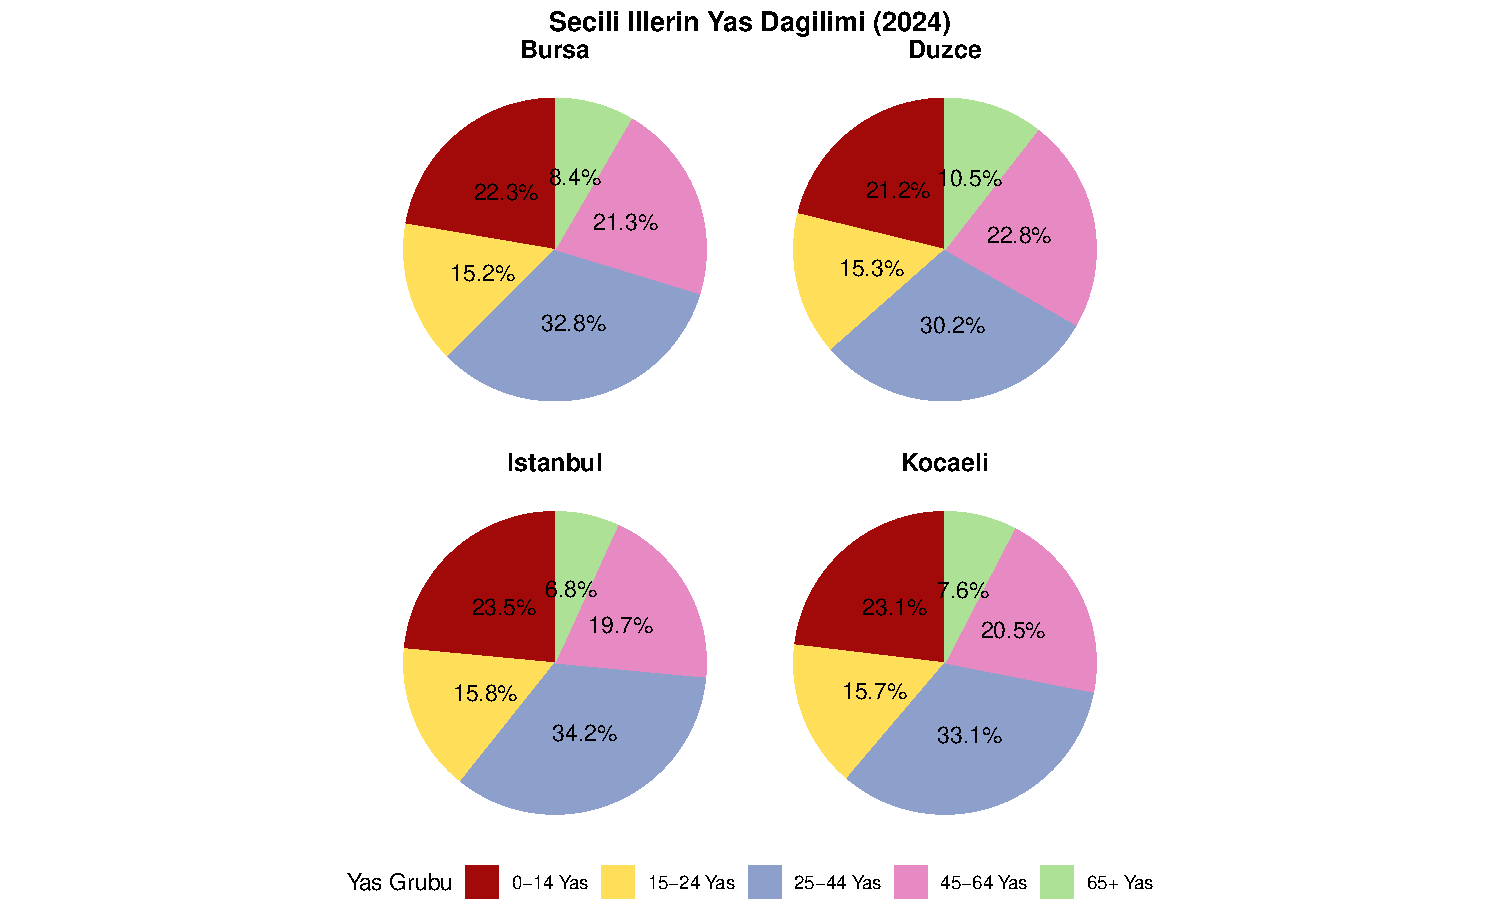
\includegraphics{cigdem_ucar_Rmarkdown_odevi_files/figure-latex/secili-iller-pasta-1.pdf}

Bu grafikler ve tablolar, Marmara ve Batı Karadeniz bölgesindeki illerin
yaş dağılımını göstermektedir. Görüldüğü üzere, Marmara bölgesindeki
illerde genç nüfus (0-24 yaş) oranı daha yüksekken, Batı Karadeniz
bölgesindeki illerde yaşlı nüfus (65+ yaş) oranı daha fazladır.

\subsection{♂️♀️ Marmara ve Batı Karadeniz İlleri Cinsiyet Verileri
(2019-2024)}\label{marmara-ve-batux131-karadeniz-illeri-cinsiyet-verileri-2019-2024}

Marmara ve Batı Karadeniz illeri cinsiyet analizi yapmak için verilere
ihtiyacımız vardı bunu da rastgele sayılardan elde ettim.

\begin{Shaded}
\begin{Highlighting}[]
\CommentTok{\# Şehirler listesi}
\NormalTok{sehirler }\OtherTok{\textless{}{-}} \FunctionTok{c}\NormalTok{(}\StringTok{"Istanbul"}\NormalTok{, }\StringTok{"Bursa"}\NormalTok{, }\StringTok{"Kocaeli"}\NormalTok{, }\StringTok{"Sakarya"}\NormalTok{, }\StringTok{"Tekirdag"}\NormalTok{, }
              \StringTok{"Zonguldak"}\NormalTok{, }\StringTok{"Bartin"}\NormalTok{, }\StringTok{"Karabuk"}\NormalTok{, }\StringTok{"Bolu"}\NormalTok{, }\StringTok{"Duzce"}\NormalTok{)}

\CommentTok{\# Yıllar}
\NormalTok{yillar }\OtherTok{\textless{}{-}} \DecValTok{2019}\SpecialCharTok{:}\DecValTok{2024}

\CommentTok{\# Veriyi oluştur}
\FunctionTok{set.seed}\NormalTok{(}\DecValTok{123}\NormalTok{) }\CommentTok{\# Rastgele sayılar için sabit bir seed değeri}
\NormalTok{veri }\OtherTok{\textless{}{-}} \FunctionTok{expand.grid}\NormalTok{(}\AttributeTok{il =}\NormalTok{ sehirler, }\AttributeTok{yil =}\NormalTok{ yillar, }\AttributeTok{cinsiyet =} \FunctionTok{c}\NormalTok{(}\StringTok{"Erkek"}\NormalTok{, }\StringTok{"Kadin"}\NormalTok{)) }\SpecialCharTok{\%\textgreater{}\%}
  \FunctionTok{mutate}\NormalTok{(}\AttributeTok{sayi =} \FunctionTok{round}\NormalTok{(}\FunctionTok{runif}\NormalTok{(}\FunctionTok{n}\NormalTok{(), }\DecValTok{500000}\NormalTok{, }\DecValTok{2000000}\NormalTok{))) }\CommentTok{\# Rastgele kişi sayısı oluştur}

\NormalTok{veri}
\end{Highlighting}
\end{Shaded}

\begin{verbatim}
##            il  yil cinsiyet    sayi
## 1    Istanbul 2019    Erkek  931366
## 2       Bursa 2019    Erkek 1682458
## 3     Kocaeli 2019    Erkek 1113465
## 4     Sakarya 2019    Erkek 1824526
## 5    Tekirdag 2019    Erkek 1910701
## 6   Zonguldak 2019    Erkek  568335
## 7      Bartin 2019    Erkek 1292158
## 8     Karabuk 2019    Erkek 1838629
## 9        Bolu 2019    Erkek 1327153
## 10      Duzce 2019    Erkek 1184922
## 11   Istanbul 2020    Erkek 1935250
## 12      Bursa 2020    Erkek 1180001
## 13    Kocaeli 2020    Erkek 1516356
## 14    Sakarya 2020    Erkek 1358950
## 15   Tekirdag 2020    Erkek  654387
## 16  Zonguldak 2020    Erkek 1849737
## 17     Bartin 2020    Erkek  869132
## 18    Karabuk 2020    Erkek  563089
## 19       Bolu 2020    Erkek  991881
## 20      Duzce 2020    Erkek 1931755
## 21   Istanbul 2021    Erkek 1834309
## 22      Bursa 2021    Erkek 1539205
## 23    Kocaeli 2021    Erkek 1460760
## 24    Sakarya 2021    Erkek 1991405
## 25   Tekirdag 2021    Erkek 1483559
## 26  Zonguldak 2021    Erkek 1562796
## 27     Bartin 2021    Erkek 1316099
## 28    Karabuk 2021    Erkek 1391213
## 29       Bolu 2021    Erkek  933740
## 30      Duzce 2021    Erkek  720670
## 31   Istanbul 2022    Erkek 1944536
## 32      Bursa 2022    Erkek 1853449
## 33    Kocaeli 2022    Erkek 1536058
## 34    Sakarya 2022    Erkek 1693201
## 35   Tekirdag 2022    Erkek  536921
## 36  Zonguldak 2022    Erkek 1216694
## 37     Bartin 2022    Erkek 1637689
## 38    Karabuk 2022    Erkek  824612
## 39       Bolu 2022    Erkek  977272
## 40      Duzce 2022    Erkek  847439
## 41   Istanbul 2023    Erkek  714200
## 42      Bursa 2023    Erkek 1121820
## 43    Kocaeli 2023    Erkek 1120586
## 44    Sakarya 2023    Erkek 1053268
## 45   Tekirdag 2023    Erkek  728667
## 46  Zonguldak 2023    Erkek  708209
## 47     Bartin 2023    Erkek  849551
## 48    Karabuk 2023    Erkek 1198944
## 49       Bolu 2023    Erkek  898959
## 50      Duzce 2023    Erkek 1786742
## 51   Istanbul 2024    Erkek  568747
## 52      Bursa 2024    Erkek 1163300
## 53    Kocaeli 2024    Erkek 1698387
## 54    Sakarya 2024    Erkek  682849
## 55   Tekirdag 2024    Erkek 1341422
## 56  Zonguldak 2024    Erkek  809797
## 57     Bartin 2024    Erkek  691297
## 58    Karabuk 2024    Erkek 1629962
## 59       Bolu 2024    Erkek 1842568
## 60      Duzce 2024    Erkek 1061694
## 61   Istanbul 2019    Kadin 1497673
## 62      Bursa 2019    Kadin  642261
## 63    Kocaeli 2019    Kadin 1075954
## 64    Sakarya 2019    Kadin  911575
## 65   Tekirdag 2019    Kadin 1721960
## 66  Zonguldak 2019    Kadin 1172775
## 67     Bartin 2019    Kadin 1715097
## 68    Karabuk 2019    Kadin 1718584
## 69       Bolu 2019    Kadin 1691513
## 70      Duzce 2019    Kadin 1159748
## 71   Istanbul 2020    Kadin 1631713
## 72      Bursa 2020    Kadin 1443832
## 73    Kocaeli 2020    Kadin 1565274
## 74    Sakarya 2020    Kadin  500937
## 75   Tekirdag 2020    Kadin 1212975
## 76  Zonguldak 2020    Kadin  830178
## 77     Bartin 2020    Kadin 1069725
## 78    Karabuk 2020    Kadin 1419157
## 79       Bolu 2020    Kadin 1027697
## 80      Duzce 2020    Kadin  666703
## 81   Istanbul 2021    Kadin  865429
## 82      Bursa 2021    Kadin 1502083
## 83    Kocaeli 2021    Kadin 1126470
## 84    Sakarya 2021    Kadin 1682294
## 85   Tekirdag 2021    Kadin  654297
## 86  Zonguldak 2021    Kadin 1152339
## 87     Bartin 2021    Kadin 1977435
## 88    Karabuk 2021    Kadin 1839577
## 89       Bolu 2021    Kadin 1829704
## 90      Duzce 2021    Kadin  762579
## 91   Istanbul 2022    Kadin  696044
## 92      Bursa 2022    Kadin 1479653
## 93    Kocaeli 2022    Kadin 1015275
## 94    Sakarya 2022    Kadin 1485137
## 95   Tekirdag 2022    Kadin  980560
## 96  Zonguldak 2022    Kadin  781537
## 97     Bartin 2022    Kadin 1673441
## 98    Karabuk 2022    Kadin  640392
## 99       Bolu 2022    Kadin 1200169
## 100     Duzce 2022    Kadin 1267258
## 101  Istanbul 2023    Kadin 1399983
## 102     Bursa 2023    Kadin  999235
## 103   Kocaeli 2023    Kadin 1232920
## 104   Sakarya 2023    Kadin 1931711
## 105  Tekirdag 2023    Kadin 1224354
## 106 Zonguldak 2023    Kadin 1835525
## 107    Bartin 2023    Kadin 1871657
## 108   Karabuk 2023    Kadin 1413102
## 109      Bolu 2023    Kadin 1116035
## 110     Duzce 2023    Kadin  720642
## 111  Istanbul 2024    Kadin 1902950
## 112     Bursa 2024    Kadin  951843
## 113   Kocaeli 2024    Kadin  591081
## 114   Sakarya 2024    Kadin 1921590
## 115  Tekirdag 2024    Kadin 1580894
## 116 Zonguldak 2024    Kadin  713441
## 117    Bartin 2024    Kadin 1323927
## 118   Karabuk 2024    Kadin 1931137
## 119      Bolu 2024    Kadin 1378225
## 120     Duzce 2024    Kadin 1106765
\end{verbatim}

\subsection{Marmara ve Batı Karadeniz de bulunan illerin cinsiyet
verilerinin makarna grafiği
gösterimi}\label{marmara-ve-batux131-karadeniz-de-bulunan-illerin-cinsiyet-verilerinin-makarna-grafiux11fi-guxf6sterimi}

Her şehir için cinsiyet bazında zaman yerinde değişim gösteren bir
makarna grafiği çiziyoruz. Renkleri manuel olarak değiştiriyoruz.

\begin{Shaded}
\begin{Highlighting}[]
\NormalTok{renk\_paleti }\OtherTok{\textless{}{-}} \FunctionTok{c}\NormalTok{(}\StringTok{"Erkek"} \OtherTok{=} \StringTok{"\#8da0cb"}\NormalTok{, }\StringTok{"Kadin"} \OtherTok{=} \StringTok{"\#a20a0a"}\NormalTok{) }\CommentTok{\# Mavi ve Kırmızı renkler}


\FunctionTok{ggplot}\NormalTok{(veri, }\FunctionTok{aes}\NormalTok{(}\AttributeTok{x =}\NormalTok{ yil, }\AttributeTok{y =}\NormalTok{ sayi, }\AttributeTok{color =}\NormalTok{ cinsiyet, }\AttributeTok{group =} \FunctionTok{interaction}\NormalTok{(il, cinsiyet))) }\SpecialCharTok{+}
  \FunctionTok{geom\_line}\NormalTok{(}\AttributeTok{size =} \FloatTok{0.8}\NormalTok{, }\AttributeTok{alpha =} \FloatTok{0.7}\NormalTok{) }\SpecialCharTok{+} 
  \FunctionTok{scale\_color\_manual}\NormalTok{(}\AttributeTok{values =}\NormalTok{ renk\_paleti) }\SpecialCharTok{+} 
  \FunctionTok{facet\_wrap}\NormalTok{(}\SpecialCharTok{\textasciitilde{}}\NormalTok{ il, }\AttributeTok{ncol =} \DecValTok{3}\NormalTok{) }\SpecialCharTok{+} 
  \FunctionTok{labs}\NormalTok{(}\AttributeTok{title =} \StringTok{"2019{-}2024 Cinsiyet Dağılımı (Makarna Grafiği)"}\NormalTok{,}
       \AttributeTok{x =} \StringTok{"Yıl"}\NormalTok{,}
       \AttributeTok{y =} \StringTok{"Kişi Sayısı"}\NormalTok{,}
       \AttributeTok{color =} \StringTok{"Cinsiyet"}\NormalTok{) }\SpecialCharTok{+}
  \FunctionTok{theme\_minimal}\NormalTok{() }\SpecialCharTok{+}
  \FunctionTok{theme}\NormalTok{(}\AttributeTok{axis.text.x =} \FunctionTok{element\_text}\NormalTok{(}\AttributeTok{angle =} \DecValTok{45}\NormalTok{, }\AttributeTok{hjust =} \DecValTok{1}\NormalTok{)) }\CommentTok{\# X eksenindeki yıl etiketlerini döndür}
\end{Highlighting}
\end{Shaded}

\begin{verbatim}
## Warning: Using `size` aesthetic for lines was deprecated in ggplot2 3.4.0.
## i Please use `linewidth` instead.
## This warning is displayed once every 8 hours.
## Call `lifecycle::last_lifecycle_warnings()` to see where this warning was
## generated.
\end{verbatim}

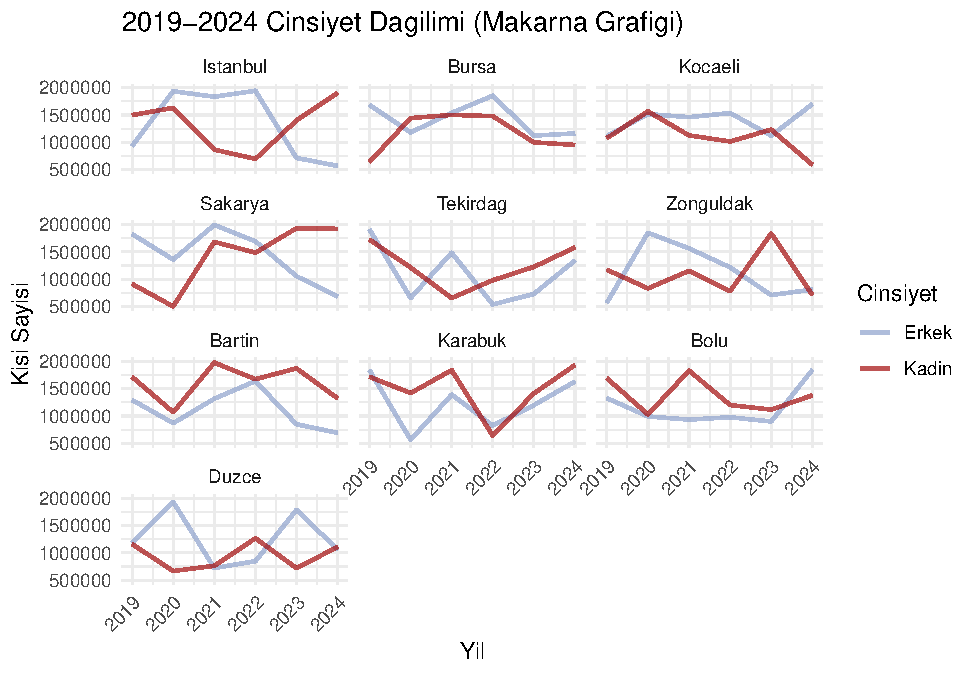
\includegraphics{cigdem_ucar_Rmarkdown_odevi_files/figure-latex/unnamed-chunk-11-1.pdf}

\subsection{Yoğunluk haritası}\label{youx11funluk-haritasux131}

\begin{Shaded}
\begin{Highlighting}[]
\FunctionTok{library}\NormalTok{(ggplot2)}
\FunctionTok{library}\NormalTok{(dplyr)}
\FunctionTok{library}\NormalTok{(tidyr) }\CommentTok{\# Veriyi pivot yapmak için}
\end{Highlighting}
\end{Shaded}

\begin{Shaded}
\begin{Highlighting}[]
\CommentTok{\# Şehirler listesi}
\NormalTok{sehirler }\OtherTok{\textless{}{-}} \FunctionTok{c}\NormalTok{(}\StringTok{"Istanbul"}\NormalTok{, }\StringTok{"Bursa"}\NormalTok{, }\StringTok{"Kocaeli"}\NormalTok{, }\StringTok{"Sakarya"}\NormalTok{, }\StringTok{"Tekirdag"}\NormalTok{, }
              \StringTok{"Zonguldak"}\NormalTok{, }\StringTok{"Bartin"}\NormalTok{, }\StringTok{"Karabuk"}\NormalTok{, }\StringTok{"Bolu"}\NormalTok{, }\StringTok{"Duzce"}\NormalTok{)}

\CommentTok{\# Yıllar}
\NormalTok{yillar }\OtherTok{\textless{}{-}} \DecValTok{2019}\SpecialCharTok{:}\DecValTok{2024}

\CommentTok{\# Veriyi oluştur}
\FunctionTok{set.seed}\NormalTok{(}\DecValTok{123}\NormalTok{) }\CommentTok{\# Rastgele sayılar için sabit bir seed değeri}
\NormalTok{veri }\OtherTok{\textless{}{-}} \FunctionTok{expand.grid}\NormalTok{(}\AttributeTok{il =}\NormalTok{ sehirler, }\AttributeTok{yil =}\NormalTok{ yillar, }\AttributeTok{cinsiyet =} \FunctionTok{c}\NormalTok{(}\StringTok{"Erkek"}\NormalTok{, }\StringTok{"Kadin"}\NormalTok{)) }\SpecialCharTok{\%\textgreater{}\%}
  \FunctionTok{mutate}\NormalTok{(}\AttributeTok{sayi =} \FunctionTok{round}\NormalTok{(}\FunctionTok{runif}\NormalTok{(}\FunctionTok{n}\NormalTok{(), }\DecValTok{500000}\NormalTok{, }\DecValTok{2000000}\NormalTok{))) }\CommentTok{\# Rastgele kişi sayısı oluştur}

\CommentTok{\# Veriyi görüntüle}
\FunctionTok{head}\NormalTok{(veri)}
\end{Highlighting}
\end{Shaded}

\begin{verbatim}
##          il  yil cinsiyet    sayi
## 1  Istanbul 2019    Erkek  931366
## 2     Bursa 2019    Erkek 1682458
## 3   Kocaeli 2019    Erkek 1113465
## 4   Sakarya 2019    Erkek 1824526
## 5  Tekirdag 2019    Erkek 1910701
## 6 Zonguldak 2019    Erkek  568335
\end{verbatim}

\begin{Shaded}
\begin{Highlighting}[]
\CommentTok{\# Veriyi pivot yap (wide format)}
\NormalTok{veri\_wide }\OtherTok{\textless{}{-}}\NormalTok{ veri }\SpecialCharTok{\%\textgreater{}\%}
  \FunctionTok{pivot\_wider}\NormalTok{(}\AttributeTok{names\_from =}\NormalTok{ cinsiyet, }\AttributeTok{values\_from =}\NormalTok{ sayi)}

\CommentTok{\# Veriyi görüntüle}
\FunctionTok{head}\NormalTok{(veri\_wide)}
\end{Highlighting}
\end{Shaded}

\begin{verbatim}
## # A tibble: 6 x 4
##   il          yil   Erkek   Kadin
##   <fct>     <int>   <dbl>   <dbl>
## 1 Istanbul   2019  931366 1497673
## 2 Bursa      2019 1682458  642261
## 3 Kocaeli    2019 1113465 1075954
## 4 Sakarya    2019 1824526  911575
## 5 Tekirdag   2019 1910701 1721960
## 6 Zonguldak  2019  568335 1172775
\end{verbatim}

yukarıda oluşturduğumuz kodlar kadın ve erkek oranlarını
tablolaştırmamızda işimize yaradı. Şimdi ise elde ettiğimiz verileri
yoğunluk haritasında göreceğiz.

\paragraph{Erkek Cinsiyet Yoğunluk
Haritası}\label{erkek-cinsiyet-youx11funluk-haritasux131}

\begin{Shaded}
\begin{Highlighting}[]
\CommentTok{\# Yoğunluk haritasını çiz}
\FunctionTok{ggplot}\NormalTok{(veri\_wide, }\FunctionTok{aes}\NormalTok{(}\AttributeTok{x =}\NormalTok{ yil, }\AttributeTok{y =}\NormalTok{ il, }\AttributeTok{fill =}\NormalTok{ Erkek)) }\SpecialCharTok{+}
  \FunctionTok{geom\_tile}\NormalTok{(}\AttributeTok{color =} \StringTok{"white"}\NormalTok{, }\AttributeTok{size =} \FloatTok{0.1}\NormalTok{) }\SpecialCharTok{+} \CommentTok{\# Kafeslerin kenarlarını beyaz yap}
  \FunctionTok{scale\_fill\_gradient}\NormalTok{(}\AttributeTok{low =} \StringTok{"\#f7fbff"}\NormalTok{, }\AttributeTok{high =} \StringTok{"\#08306b"}\NormalTok{) }\SpecialCharTok{+} \CommentTok{\# Renk skalası}
  \FunctionTok{labs}\NormalTok{(}\AttributeTok{title =} \StringTok{"Erkek Cinsiyet Yoğunluk Haritası"}\NormalTok{,}
       \AttributeTok{x =} \StringTok{"Yıl"}\NormalTok{,}
       \AttributeTok{y =} \StringTok{"Şehir"}\NormalTok{,}
       \AttributeTok{fill =} \StringTok{"Kişi Sayısı"}\NormalTok{) }\SpecialCharTok{+}
  \FunctionTok{theme\_minimal}\NormalTok{() }\SpecialCharTok{+}
  \FunctionTok{theme}\NormalTok{(}\AttributeTok{axis.text.x =} \FunctionTok{element\_text}\NormalTok{(}\AttributeTok{angle =} \DecValTok{45}\NormalTok{, }\AttributeTok{hjust =} \DecValTok{1}\NormalTok{)) }\CommentTok{\# X eksenindeki yıl etiketlerini döndür}
\end{Highlighting}
\end{Shaded}

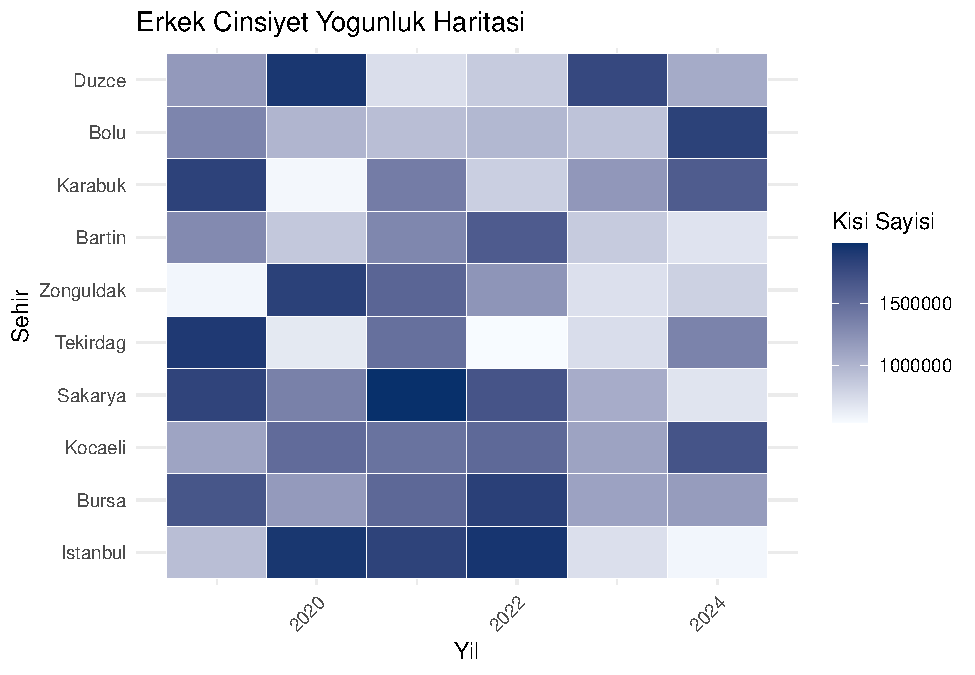
\includegraphics{cigdem_ucar_Rmarkdown_odevi_files/figure-latex/unnamed-chunk-15-1.pdf}

\paragraph{Kadın Cinsiyet Yoğunluk
Haritası}\label{kadux131n-cinsiyet-youx11funluk-haritasux131}

\begin{Shaded}
\begin{Highlighting}[]
\CommentTok{\# Kadın için yoğunluk haritasını çiz}
\FunctionTok{ggplot}\NormalTok{(veri\_wide, }\FunctionTok{aes}\NormalTok{(}\AttributeTok{x =}\NormalTok{ yil, }\AttributeTok{y =}\NormalTok{ il, }\AttributeTok{fill =}\NormalTok{ Kadin)) }\SpecialCharTok{+}
  \FunctionTok{geom\_tile}\NormalTok{(}\AttributeTok{color =} \StringTok{"white"}\NormalTok{, }\AttributeTok{size =} \FloatTok{0.1}\NormalTok{) }\SpecialCharTok{+} \CommentTok{\# Kafeslerin kenarlarını beyaz yap}
  \FunctionTok{scale\_fill\_gradient}\NormalTok{(}\AttributeTok{low =} \StringTok{"\#fff5f0"}\NormalTok{, }\AttributeTok{high =} \StringTok{"\#67000d"}\NormalTok{) }\SpecialCharTok{+} \CommentTok{\# Renk skalası}
  \FunctionTok{labs}\NormalTok{(}\AttributeTok{title =} \StringTok{"Kadın Cinsiyet Yoğunluk Haritası"}\NormalTok{,}
       \AttributeTok{x =} \StringTok{"Yıl"}\NormalTok{,}
       \AttributeTok{y =} \StringTok{"Şehir"}\NormalTok{,}
       \AttributeTok{fill =} \StringTok{"Kişi Sayısı"}\NormalTok{) }\SpecialCharTok{+}
  \FunctionTok{theme\_minimal}\NormalTok{() }\SpecialCharTok{+}
  \FunctionTok{theme}\NormalTok{(}\AttributeTok{axis.text.x =} \FunctionTok{element\_text}\NormalTok{(}\AttributeTok{angle =} \DecValTok{45}\NormalTok{, }\AttributeTok{hjust =} \DecValTok{1}\NormalTok{)) }\CommentTok{\# X eksenindeki yıl etiketlerini döndür}
\end{Highlighting}
\end{Shaded}

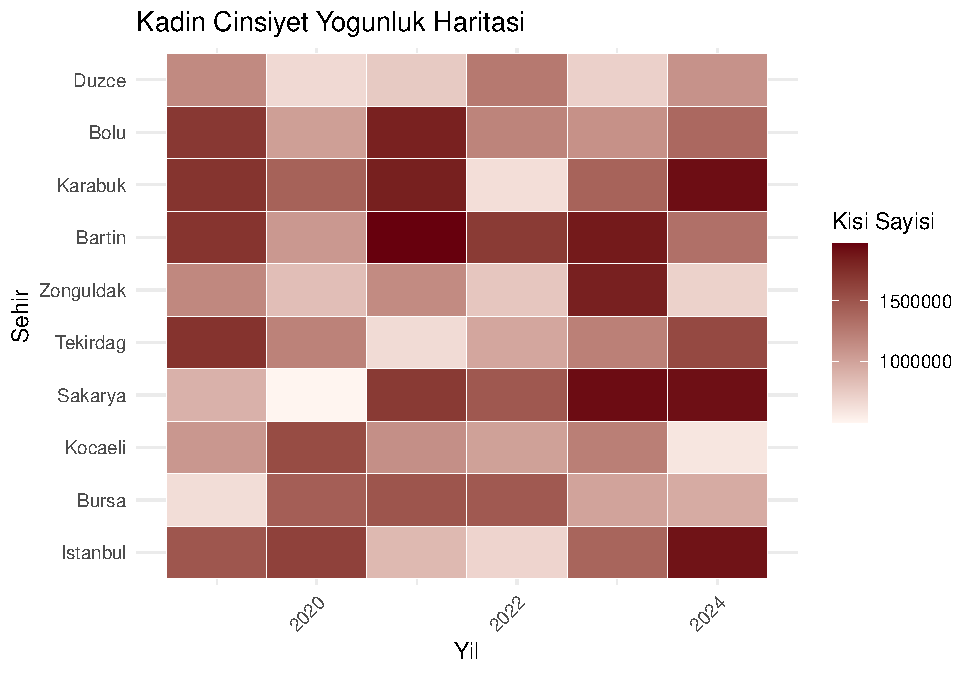
\includegraphics{cigdem_ucar_Rmarkdown_odevi_files/figure-latex/unnamed-chunk-16-1.pdf}

\subsection{kelime bulutu}\label{kelime-bulutu}

Ek olarak Batı Karadeniz ve Marmara bölgelerinde baz aldığımız illeri
içeren bir kelime bulutu oluşturdum.

⇓⇓⇓⇓⇓⇓⇓⇓⇓⇓⇓⇓⇓⇓⇓⇓⇓⇓⇓⇓⇓⇓⇓⇓⇓⇓⇓⇓

\begin{Shaded}
\begin{Highlighting}[]
\FunctionTok{library}\NormalTok{(ggwordcloud)}
\FunctionTok{library}\NormalTok{(ggplot2)}
\FunctionTok{library}\NormalTok{(showtext)}
\end{Highlighting}
\end{Shaded}

\begin{verbatim}
## Zorunlu paket yükleniyor: sysfonts
\end{verbatim}

\begin{verbatim}
## Zorunlu paket yükleniyor: showtextdb
\end{verbatim}

\begin{Shaded}
\begin{Highlighting}[]
\FunctionTok{library}\NormalTok{(RColorBrewer)}
\end{Highlighting}
\end{Shaded}

\begin{Shaded}
\begin{Highlighting}[]
\CommentTok{\# Karadeniz Bölgesi şehirleri}
\NormalTok{karadeniz\_sehirleri }\OtherTok{\textless{}{-}} \FunctionTok{c}\NormalTok{(}\StringTok{"Bartın"}\NormalTok{, }\StringTok{"Bolu"}\NormalTok{, }\StringTok{"Düzce"}\NormalTok{, }\StringTok{"Karabük"}\NormalTok{, }\StringTok{"Kastamonu"}\NormalTok{, }\StringTok{"Zonguldak"}\NormalTok{)}

\CommentTok{\# Marmara Bölgesi şehirleri}
\NormalTok{marmara\_sehirleri }\OtherTok{\textless{}{-}} \FunctionTok{c}\NormalTok{(}\StringTok{"Balıkesir"}\NormalTok{, }\StringTok{"Bilecik"}\NormalTok{, }\StringTok{"Bursa"}\NormalTok{, }\StringTok{"Çanakkale"}\NormalTok{, }\StringTok{"Edirne"}\NormalTok{, }\StringTok{"İstanbul"}\NormalTok{,}
                        \StringTok{"Kırklareli"}\NormalTok{, }\StringTok{"Kocaeli"}\NormalTok{, }\StringTok{"Sakarya"}\NormalTok{, }\StringTok{"Tekirdağ"}\NormalTok{, }\StringTok{"Yalova"}\NormalTok{)}

\CommentTok{\# Tüm şehirleri birleştir}
\NormalTok{tum\_sehirler }\OtherTok{\textless{}{-}} \FunctionTok{c}\NormalTok{(karadeniz\_sehirleri, marmara\_sehirleri)}

\CommentTok{\# Şehirlerin kelime sıklığını rastgele belirleyelim}
\FunctionTok{set.seed}\NormalTok{(}\DecValTok{123}\NormalTok{)}
\NormalTok{frekanslar }\OtherTok{\textless{}{-}} \FunctionTok{sample}\NormalTok{(}\DecValTok{10}\SpecialCharTok{:}\DecValTok{50}\NormalTok{, }\FunctionTok{length}\NormalTok{(tum\_sehirler), }\AttributeTok{replace =} \ConstantTok{TRUE}\NormalTok{)  }\CommentTok{\# 10{-}50 arası rastgele frekans}
\NormalTok{renkler }\OtherTok{\textless{}{-}} \FunctionTok{sample}\NormalTok{(}\FunctionTok{brewer.pal}\NormalTok{(}\DecValTok{8}\NormalTok{, }\StringTok{"Dark2"}\NormalTok{), }\FunctionTok{length}\NormalTok{(tum\_sehirler), }\AttributeTok{replace =} \ConstantTok{TRUE}\NormalTok{)  }\CommentTok{\# Rastgele renk seçimi}
\NormalTok{aci }\OtherTok{\textless{}{-}} \FunctionTok{sample}\NormalTok{(}\FunctionTok{seq}\NormalTok{(}\SpecialCharTok{{-}}\DecValTok{45}\NormalTok{, }\DecValTok{45}\NormalTok{, }\AttributeTok{by =} \DecValTok{15}\NormalTok{), }\FunctionTok{length}\NormalTok{(tum\_sehirler), }\AttributeTok{replace =} \ConstantTok{TRUE}\NormalTok{)  }\CommentTok{\# Rastgele açılar}

\CommentTok{\# Veri çerçevesini oluştur}
\NormalTok{sehir\_frekans }\OtherTok{\textless{}{-}} \FunctionTok{data.frame}\NormalTok{(}
  \AttributeTok{Sehir =}\NormalTok{ tum\_sehirler,}
  \AttributeTok{Frekans =}\NormalTok{ frekanslar,}
  \AttributeTok{Renk =}\NormalTok{ renkler,}
  \AttributeTok{Aci =}\NormalTok{ aci}
\NormalTok{)}

\CommentTok{\# Veriyi kontrol edelim}
\FunctionTok{print}\NormalTok{(sehir\_frekans)}
\end{Highlighting}
\end{Shaded}

\begin{verbatim}
##         Sehir Frekans    Renk Aci
## 1      Bartın      40 #A6761D -45
## 2        Bolu      24 #D95F02 -45
## 3       Düzce      23 #1B9E77 -30
## 4     Karabük      12 #E6AB02  45
## 5   Kastamonu      46 #7570B3 -15
## 6   Zonguldak      23 #E7298A   0
## 7   Balıkesir      34 #E6AB02  15
## 8     Bilecik      35 #1B9E77  45
## 9       Bursa      36 #7570B3  15
## 10  Çanakkale      14 #A6761D -15
## 11     Edirne      36 #66A61E  30
## 12   İstanbul      37 #E7298A -45
## 13 Kırklareli      18 #A6761D -30
## 14    Kocaeli      38 #666666  15
## 15    Sakarya      44 #D95F02  15
## 16   Tekirdağ      17 #66A61E   0
## 17     Yalova      35 #A6761D  45
\end{verbatim}

\begin{Shaded}
\begin{Highlighting}[]
\CommentTok{\# Türkçe fontları ekleyelim}
\FunctionTok{font\_add\_google}\NormalTok{(}\StringTok{"Open Sans"}\NormalTok{, }\StringTok{"opensans"}\NormalTok{)}
\FunctionTok{showtext\_auto}\NormalTok{()}
\end{Highlighting}
\end{Shaded}

\begin{Shaded}
\begin{Highlighting}[]
\FunctionTok{ggplot}\NormalTok{(sehir\_frekans, }\FunctionTok{aes}\NormalTok{(}\AttributeTok{label =}\NormalTok{ Sehir, }\AttributeTok{size =}\NormalTok{ Frekans, }\AttributeTok{color =}\NormalTok{ Renk, }\AttributeTok{angle =}\NormalTok{ Aci)) }\SpecialCharTok{+}
  \FunctionTok{geom\_text\_wordcloud}\NormalTok{(}\AttributeTok{family =} \StringTok{"opensans"}\NormalTok{, }\AttributeTok{fontface =} \StringTok{"bold"}\NormalTok{) }\SpecialCharTok{+}  \CommentTok{\# Türkçe destekli font}
  \FunctionTok{scale\_size\_area}\NormalTok{(}\AttributeTok{max\_size =} \DecValTok{15}\NormalTok{) }\SpecialCharTok{+}  \CommentTok{\# Kelime boyutlarını belirle}
  \FunctionTok{scale\_color\_identity}\NormalTok{() }\SpecialCharTok{+}  \CommentTok{\# Renkleri doğrudan kullan}
  \FunctionTok{theme\_minimal}\NormalTok{() }\SpecialCharTok{+}
  \FunctionTok{ggtitle}\NormalTok{(}\StringTok{"Batı Karadeniz ve Marmara Şehirleri Kelime Bulutu"}\NormalTok{) }\SpecialCharTok{+}
  \FunctionTok{theme}\NormalTok{(}\AttributeTok{plot.title =} \FunctionTok{element\_text}\NormalTok{(}\AttributeTok{size =} \DecValTok{16}\NormalTok{, }\AttributeTok{face =} \StringTok{"bold"}\NormalTok{))}
\end{Highlighting}
\end{Shaded}

\begin{verbatim}
## Warning in grid.Call.graphics(C_text, as.graphicsAnnot(x$label), x$x, x$y, :
## font family not found in Windows font database
## Warning in grid.Call.graphics(C_text, as.graphicsAnnot(x$label), x$x, x$y, :
## font family not found in Windows font database
## Warning in grid.Call.graphics(C_text, as.graphicsAnnot(x$label), x$x, x$y, :
## font family not found in Windows font database
## Warning in grid.Call.graphics(C_text, as.graphicsAnnot(x$label), x$x, x$y, :
## font family not found in Windows font database
## Warning in grid.Call.graphics(C_text, as.graphicsAnnot(x$label), x$x, x$y, :
## font family not found in Windows font database
## Warning in grid.Call.graphics(C_text, as.graphicsAnnot(x$label), x$x, x$y, :
## font family not found in Windows font database
## Warning in grid.Call.graphics(C_text, as.graphicsAnnot(x$label), x$x, x$y, :
## font family not found in Windows font database
## Warning in grid.Call.graphics(C_text, as.graphicsAnnot(x$label), x$x, x$y, :
## font family not found in Windows font database
## Warning in grid.Call.graphics(C_text, as.graphicsAnnot(x$label), x$x, x$y, :
## font family not found in Windows font database
## Warning in grid.Call.graphics(C_text, as.graphicsAnnot(x$label), x$x, x$y, :
## font family not found in Windows font database
## Warning in grid.Call.graphics(C_text, as.graphicsAnnot(x$label), x$x, x$y, :
## font family not found in Windows font database
## Warning in grid.Call.graphics(C_text, as.graphicsAnnot(x$label), x$x, x$y, :
## font family not found in Windows font database
## Warning in grid.Call.graphics(C_text, as.graphicsAnnot(x$label), x$x, x$y, :
## font family not found in Windows font database
## Warning in grid.Call.graphics(C_text, as.graphicsAnnot(x$label), x$x, x$y, :
## font family not found in Windows font database
## Warning in grid.Call.graphics(C_text, as.graphicsAnnot(x$label), x$x, x$y, :
## font family not found in Windows font database
## Warning in grid.Call.graphics(C_text, as.graphicsAnnot(x$label), x$x, x$y, :
## font family not found in Windows font database
## Warning in grid.Call.graphics(C_text, as.graphicsAnnot(x$label), x$x, x$y, :
## font family not found in Windows font database
## Warning in grid.Call.graphics(C_text, as.graphicsAnnot(x$label), x$x, x$y, :
## font family not found in Windows font database
## Warning in grid.Call.graphics(C_text, as.graphicsAnnot(x$label), x$x, x$y, :
## font family not found in Windows font database
## Warning in grid.Call.graphics(C_text, as.graphicsAnnot(x$label), x$x, x$y, :
## font family not found in Windows font database
## Warning in grid.Call.graphics(C_text, as.graphicsAnnot(x$label), x$x, x$y, :
## font family not found in Windows font database
## Warning in grid.Call.graphics(C_text, as.graphicsAnnot(x$label), x$x, x$y, :
## font family not found in Windows font database
## Warning in grid.Call.graphics(C_text, as.graphicsAnnot(x$label), x$x, x$y, :
## font family not found in Windows font database
## Warning in grid.Call.graphics(C_text, as.graphicsAnnot(x$label), x$x, x$y, :
## font family not found in Windows font database
## Warning in grid.Call.graphics(C_text, as.graphicsAnnot(x$label), x$x, x$y, :
## font family not found in Windows font database
## Warning in grid.Call.graphics(C_text, as.graphicsAnnot(x$label), x$x, x$y, :
## font family not found in Windows font database
## Warning in grid.Call.graphics(C_text, as.graphicsAnnot(x$label), x$x, x$y, :
## font family not found in Windows font database
## Warning in grid.Call.graphics(C_text, as.graphicsAnnot(x$label), x$x, x$y, :
## font family not found in Windows font database
## Warning in grid.Call.graphics(C_text, as.graphicsAnnot(x$label), x$x, x$y, :
## font family not found in Windows font database
## Warning in grid.Call.graphics(C_text, as.graphicsAnnot(x$label), x$x, x$y, :
## font family not found in Windows font database
## Warning in grid.Call.graphics(C_text, as.graphicsAnnot(x$label), x$x, x$y, :
## font family not found in Windows font database
## Warning in grid.Call.graphics(C_text, as.graphicsAnnot(x$label), x$x, x$y, :
## font family not found in Windows font database
\end{verbatim}

\begin{verbatim}
## Warning in wordcloud_boxes(data_points = points_valid_first, boxes = boxes, :
## Some words could not fit on page. They have been placed at their original
## positions.
\end{verbatim}

\includegraphics{cigdem_ucar_Rmarkdown_odevi_files/figure-latex/unnamed-chunk-20-1.pdf}

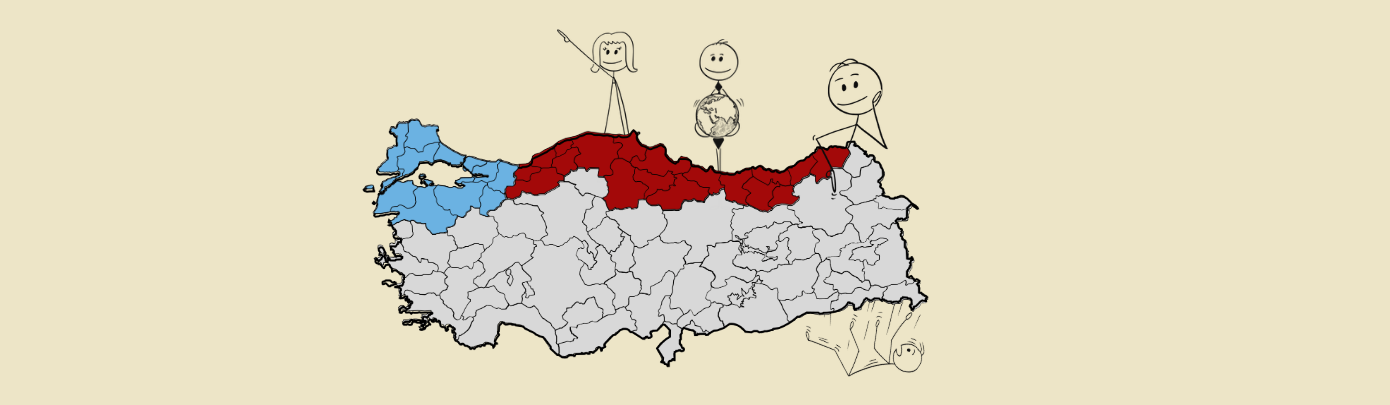
\includegraphics[width=19.31in]{son_goruntu}

Tarayıcınız ses dosyasını desteklemiyor.

\end{document}
